\chapter[Reciprocity through the Swap]{Reciprocity through the Swap:\\ Thorin Measures, Wald Couples\\ and van Dantzig Duality}\label{ch:recip}

Langlands reciprocity asserts that two very different kinds of object carry the same information: a Galois representation $\rho$, known through the conjugacy classes of its Frobenius elements, one prime at a time, and an automorphic representation $\pi$, a harmonic object on an adelic quotient, known through Hecke eigenvalues, Fourier coefficients and spectral data. Reciprocity says that $L(s,\rho)=L(s,\pi)$. The difficulty is that Frobenius data are local and arithmetic, while automorphy is a global symmetry visible only to harmonic analysis.

This chapter proposes to bring the Thorin framework of Chapters~\ref{ch:10b} to \ref{ch:10d} to bear on reciprocity, starting from one observation: the completed $L$ function is a single function with two faces. On the Euler half line $\operatorname{Re}s>1$ it is an Euler product, a statement about primes, the Galois side; on the critical line it is the Mellin transform of an automorphic form, the automorphic side. Three devices from those chapters pass between the faces: the explicit formula with the $2\sin^2$ transport of Lemma~\ref{lem:10dsin2}, which swaps the primes for the zeros; the van Dantzig involution, which exchanges the critical line with the real axis; and the Wald couple of Definition~\ref{def:10dwald}, which under GRH pairs a variable built from the automorphic form with a variable built from the Euler product. Read through them, modularity at level one becomes a symmetry statement about a P\'olya kernel, and holomorphy together with GRH becomes a positivity statement about a measure and a continuation statement about generalized gamma convolutions.

Before the proposal, three sections restate parts of reciprocity in the language of probability. Section~\ref{sec:recipgauss} derives quadratic reciprocity, Gauss's sign and the functional equations of even Dirichlet $L$ functions from the characteristic function of the normal law, and proves the theta transformation a second time by Fej\'er positivity: the swap for the circle, the model for everything after it. Section~\ref{sec:reciplaw} puts Galois and automorphic representations on one probability space, where reciprocity is almost sure equality and its uniqueness statements are Hilbert space inequalities. Section~\ref{sec:recipgammaproc} replaces that space by the zeta distributed random integer, whose Frobenius labelled factorisation converges to a Gamma process; reciprocity laws become the vanishing of Thorin measures, and the drift of the split primes is Ihara's Euler Kronecker constant over the degree, up to finitely many Euler factors and a prime power term.

We do not prove new cases of reciprocity. We prove the results that make the proposal precise: a symmetry criterion for modularity at level one; a Gamma limit law that detects irreducibility; a complete monotonicity criterion for holomorphy together with GRH, computed from Frobenius traces, the conductor and the gamma factor, with which finitely many certified inequalities can disprove them but are not known to verify them to any finite height; a rigidity statement showing that the swap sees every single prime; and a Thorin form of Hecke's converse theorem. We test the criteria numerically on a two dimensional Artin representation of conductor $23$ (Example~\ref{ex:ch3cubic}) and on Ramanujan's $\Delta$. Proposition~\ref{prop:01limits} showed that no argument which uses only the limiting distribution of Frobenius data can prove reciprocity; the criteria of Sections~\ref{sec:recipfaces}, \ref{sec:recipswap} and \ref{sec:recipvdp} see the individual primes, while the limit laws of Sections~\ref{sec:reciplaw}, \ref{sec:recipgammaproc} and \ref{sec:recipgalois} do not. Figure~\ref{fig:recipswap} summarises the scheme.

\begin{figure}[t]
\centering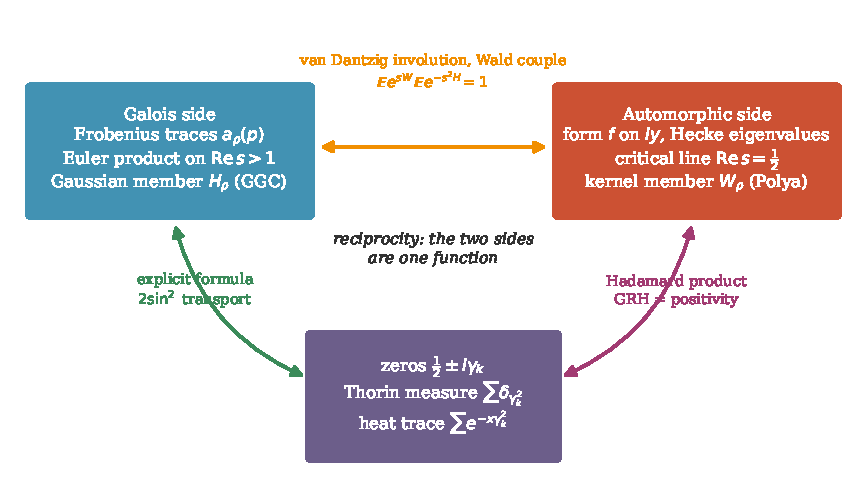
\includegraphics[width=\textwidth]{figs/recip_swap.pdf}
\caption{One function, two faces. The Euler product on $\operatorname{Re}s>1$ carries the Galois data, the Mellin transform on the critical line carries the automorphic form, and the zeros sit between them. The explicit formula with the $2\sin^2$ transport, the Hadamard product, and the van Dantzig involution with its Wald couple pass between the three.}\label{fig:recipswap}
\end{figure}

\section{The reciprocity problem}\label{sec:recipproblem}

Let $\rho$ be an Artin representation of $\Gal(\overline\Q/\Q)$ on an $n$ dimensional complex vector space $V$ or, more generally, a geometric $\ell$ adic representation on an $n$ dimensional $\overline\Q_\ell$ vector space $V$, pure of weight $w$, made complex through a fixed isomorphism $\overline\Q_\ell\cong\C$. Its gamma factor $\gamma(s,\rho)$ is determined by the Hodge numbers and the action of complex conjugation, and $N_\rho$ is its conductor. For $p$ unramified put $a_\rho(p^m)=\tr\rho(\Frob_p^m)$. In the unitary normalisation ($s$ shifted by $w/2$; at $p=\ell$ the local factor is that of the associated Weil Deligne representation) the Euler product
\[
L(s,\rho)=\prod_p\det\bigl(1-\rho(\Frob_p)p^{-s}\bigm|V^{I_p}\bigr)^{-1}
\]
converges absolutely for $\operatorname{Re}s>1$, and $\Lambda(s,\rho)=N_\rho^{s/2}\gamma(s,\rho)L(s,\rho)$ is its completion (the factor $N_\rho^{s/2}$ is kept out of $\gamma(s,\rho)$, unlike in Appendix~\ref{app:A}). Everything in $\Lambda(s,\rho)$ for $\operatorname{Re}s>1$ is Galois data: Frobenius traces, the conductor and the gamma factor. For Artin representations, Brauer's induction theorem \cite{brauer1947} gives meromorphic continuation and the functional equation $\Lambda(s,\rho)=\varepsilon(\rho)\Lambda(1-s,\check\rho)$; Artin's conjecture \cite{artin1924} asserts that $\Lambda(s,\rho)$ is entire when $\rho$ has no trivial constituent.

\begin{conjecture}[Langlands reciprocity \cite{langlands1970}]\label{conj:recip}\index{reciprocity conjecture}
For every irreducible $\rho$ as above there is a cuspidal automorphic representation $\pi$ of $\GL_n(\A_\Q)$ with $L(s,\rho_p)=L(s,\pi_p)$ for every place $p$.
\end{conjecture}

For $n=1$ this is class field theory (Artin's reciprocity law \cite{artin1927}). For $n=2$ it is known for Artin representations with solvable image, odd or even, by Hecke, Langlands and Tunnell \cite{langlands1980,tunnell1981}, for all odd ones as a consequence of Serre's conjecture, proved by Khare and Wintenberger \cite{kharewintenberger2009,kharewintenberger2009b} with work of Kisin \cite{kisin2009}, and for elliptic curves over $\Q$ by Wiles, Taylor and Wiles, and Breuil, Conrad, Diamond and Taylor \cite{wiles1995,taylorwiles1995,bcdt2001}. Potential automorphy \cite{hsbt2010,blght2011} gave meromorphic continuation and functional equations for the symmetric powers of holomorphic newforms, and Newton and Thorne \cite{newtonthorne2021,newtonthorne2021b} proved them automorphic for newforms of weight at least two without complex multiplication (Chapter~\ref{ch:03}). In dimension two the even icosahedral case is open.

The analytic route to reciprocity runs through converse theorems.\index{converse theorem} Hecke \cite{hecke1936} showed that a Dirichlet series whose completion is entire, bounded in vertical strips and satisfies the level one functional equation comes from a modular form for $\SL_2(\Z)$ (Section~\ref{sec:02mellin}). Weil \cite{weil1967} added twists by Dirichlet characters to reach $\Gamma_0(N)$; Jacquet and Langlands \cite{jacquetlanglands1970} recast this for $\GL_2$, and Cogdell and Piatetski Shapiro \cite{cogdellps1994} extended it to $\GL_n$, with twists by cuspidal representations $\pi'$ of $\GL_m$, $m\le n-1$. So, once the local Langlands correspondence has fixed the local components of the candidate $\pi$, reciprocity for $\rho$ follows from \emph{analytic} properties of the twisted $L$ functions $L(s,\rho\times\pi')$: continuation, holomorphy, boundedness and functional equations (Open Problem~\ref{op:inverse} asks for a probabilistic counterpart of these theorems). Booker \cite{booker2006} turned this into a computation, verifying Artin's conjecture up to a finite height for some nonmonomial representations with $A_5$ and $S_5$ image (Section~\ref{sec:recipswap}).

\section{Quadratic reciprocity from the Gaussian law}\label{sec:recipgauss}

For quadratic characters the analytic content of reciprocity is one probabilistic fact: the characteristic function of a normal law is a Gaussian. Here it is applied to a single random variable, the position at a fixed time of a Brownian motion wrapped around a circle. None of the theorems of this section is new, apart from the explicit bounds (i) and (ii) of Theorem~\ref{thm:recipheat}, which are elementary; the route shows which part of the classical reciprocity laws is probability.

\begin{lemma}[wrapped Gaussian]\label{lem:recipwrap}\index{Poisson summation}
For $x>0$ and real $y$,
\[
\sum_{k\in\Z}e^{-xk^2+iky}=\sqrt{\frac\pi x}\,\sum_{n\in\Z}e^{-(y+2\pi n)^2/(4x)} .
\]
\end{lemma}

\begin{proof}
Let $Y\sim N(0,2x)$, with density $\varphi(y)=(4\pi x)^{-1/2}e^{-y^2/(4x)}$, and let $\varphi_{2\pi}(y)=\sum_n\varphi(y+2\pi n)$ be the density of $Y$ reduced modulo $2\pi$. The series converges uniformly on compact sets, so $\varphi_{2\pi}$ is continuous and $2\pi$ periodic, and its Fourier coefficients are $\int_0^{2\pi}\varphi_{2\pi}(y)e^{-iky}dy=\E e^{-ikY}=e^{-xk^2}$. These are absolutely summable, so the Fourier series of $\varphi_{2\pi}$ converges uniformly, and by Fej\'er's theorem its sum is $\varphi_{2\pi}$: $\varphi_{2\pi}(y)=(2\pi)^{-1}\sum_ke^{-xk^2}e^{iky}$ for every $y$. Multiplying by $2\pi$ gives the lemma.
\end{proof}

Put $\theta(\tau)=\sum_{n\in\Z}e^{\pi in^2\tau}$ for $\operatorname{Im}\tau>0$.

\begin{theorem}[theta transformation]\label{thm:reciptheta}\index{theta function}
$\theta(-1/\tau)=\sqrt{\tau/i}\;\theta(\tau)$, with the principal branch of the square root.
\end{theorem}

\begin{proof}
Lemma~\ref{lem:recipwrap} with $y=0$ and $x=\pi t$ gives $\theta(it)=t^{-1/2}\theta(i/t)$ for $t>0$, which is the claim on the imaginary axis, since $-1/(it)=i/t$ and $\sqrt{it/i}=\sqrt t$. Both sides are holomorphic on the upper half plane, because $\tau/i$ has positive real part there, so they agree everywhere.
\end{proof}

We need one elementary estimate. If $h\in C^1(\R)$ with $h$ and $h'$ integrable, then for $t_0\in\R$ and $\eta>0$,
\begin{equation}\label{eq:recipriemann}
\Bigl|\eta\sum_{m\in\Z}h(t_0+m\eta)-\int_{\R}h\Bigr|\le\eta\int_{\R}|h'| ,
\end{equation}
because on each interval $[t_0+m\eta,t_0+(m+1)\eta]$ the difference between $\eta h(t_0+m\eta)$ and the integral of $h$ is at most $\eta$ times the integral of $|h'|$ over that interval.

For integers $a,c\ge1$ with $ac$ even put
\[
S(a,c)=\sum_{n\bmod c}e^{\pi ian^2/c}=c\,\E e^{\pi iaU^2/c},\qquad U\text{ uniform on }\Z/c\Z .
\]
The summand depends only on $n$ modulo $c$, because $a(n+c)^2/c=an^2/c+2an+ac$ and $ac$ is even.

\begin{theorem}[reciprocity for Gauss sums; Schaar, Landsberg]\label{thm:recipls}\index{Gauss sum}
For integers $a,c\ge1$ with $ac$ even,
\[
\frac1{\sqrt c}\,S(a,c)=\frac{e^{\pi i/4}}{\sqrt a}\;\overline{S(c,a)} .
\]
\end{theorem}

\begin{proof}
Let $\tau=a/c+i\varepsilon$ with $\varepsilon>0$; we let $\varepsilon\downarrow0$, so that $\theta(\tau)/\theta(i\varepsilon)$ is the characteristic function of the square of a discrete Gaussian of variance of order $\varepsilon^{-1}$, evaluated at $\pi a/c$. Grouping $n$ by its residue $r$ modulo $c$,
\[
\theta(\tau)=\sum_{r\bmod c}e^{\pi iar^2/c}\sum_{m\in\Z}e^{-\pi\varepsilon(r+mc)^2}.
\]
By \eqref{eq:recipriemann} with $h(u)=e^{-\pi u^2}$ and $\eta=c\sqrt\varepsilon$, $\sqrt\varepsilon\sum_me^{-\pi\varepsilon(r+mc)^2}\to1/c$, so $\sqrt\varepsilon\,\theta(\tau)\to S(a,c)/c$: the discrete Gaussian reduced modulo $c$ becomes uniform.

On the other side, $-1/\tau=-c/a+w$ with $w=i\delta/(1+i\kappa)$, $\delta=c^2\varepsilon/a^2$ and $\kappa=c\varepsilon/a$. Hence $e^{\pi in^2(-1/\tau)}=e^{-\pi icn^2/a}e^{-\pi\delta\beta n^2}$ with $\beta=(1+i\kappa)^{-1}$, and the first factor depends only on $n$ modulo $a$. Grouping by residues modulo $a$ and applying \eqref{eq:recipriemann} to $h_\beta(u)=e^{-\pi\beta u^2}$ with $\eta=a\sqrt\delta$, where $\int|h_\beta'|$ is bounded for $|\kappa|\le1$ and $\int h_\beta=\beta^{-1/2}\to1$, we get $\sqrt\delta\,\theta(-1/\tau)\to\overline{S(c,a)}/a$. Since $\sqrt\delta=(c/a)\sqrt\varepsilon$, this says $\sqrt\varepsilon\,\theta(-1/\tau)\to\overline{S(c,a)}/c$.

Now multiply the identity of Theorem~\ref{thm:reciptheta} by $\sqrt\varepsilon$ and let $\varepsilon\downarrow0$. Since $\sqrt{\tau/i}\to\sqrt{a/c}\,e^{-\pi i/4}$, we get $\overline{S(c,a)}/c=\sqrt{a/c}\,e^{-\pi i/4}S(a,c)/c$, which is the theorem.
\end{proof}

\begin{corollary}[Gauss's sign]\label{cor:recipgausssign}
For odd $m\ge1$, $g(m)=\sum_{n\bmod m}e^{2\pi in^2/m}$ equals $\sqrt m$ if $m\equiv1\bmod4$ and $i\sqrt m$ if $m\equiv3\bmod4$.
\end{corollary}

\begin{proof}
Take $a=2$, $c=m$: $g(m)=S(2,m)=\sqrt{m/2}\,e^{\pi i/4}(1+e^{-\pi im/2})$. For $m\equiv1\bmod4$, $1+e^{-\pi im/2}=1-i=\sqrt2e^{-\pi i/4}$; for $m\equiv3\bmod4$ it is $1+i=\sqrt2e^{\pi i/4}$.
\end{proof}

Gauss conjectured the sign in 1801, found a proof only in 1805 and published it in 1811 \cite{gauss1811}. Here it is the limit point of the curve $\varepsilon\mapsto\sqrt\varepsilon\,\theta(2/m+i\varepsilon)$ (Figure~\ref{fig:recipgauss}, left).

\begin{corollary}[quadratic reciprocity]\label{cor:recipqr}\index{quadratic reciprocity}
For distinct odd primes $p,q$,
\[
\Bigl(\frac pq\Bigr)\Bigl(\frac qp\Bigr)=(-1)^{\frac{p-1}2\frac{q-1}2},\qquad \Bigl(\frac{-1}p\Bigr)=(-1)^{\frac{p-1}2},\qquad\Bigl(\frac2p\Bigr)=(-1)^{\frac{p^2-1}8}.
\]
\end{corollary}

\begin{proof}
For $p\nmid k$ put $g_k(p)=\sum_{n\bmod p}e^{2\pi ikn^2/p}$. Since $n^2\equiv b$ has $1+(\frac bp)$ solutions, $g_k(p)=\sum_b(\frac bp)e^{2\pi ikb/p}=(\frac kp)g(p)$ after substituting $b\mapsto k^{-1}b$. By Proposition~\ref{prop:recipgood} below, $g(pq)=g_q(p)g_p(q)=(\frac qp)(\frac pq)g(p)g(q)$. Write $g(m)=\omega_m\sqrt m$ with $\omega_m\in\{1,i\}$ from Corollary~\ref{cor:recipgausssign}, which applies to the composite $m=pq$. Then $(\frac pq)(\frac qp)=\omega_{pq}/(\omega_p\omega_q)$, which is $1/i^2=-1$ when $p\equiv q\equiv3\bmod4$ and $1$ otherwise.

For the first supplement, $\overline{g(p)}=g_{-1}(p)=(\frac{-1}p)g(p)$, and $g(p)$ is real exactly when $p\equiv1\bmod4$. For the second, Theorem~\ref{thm:recipls} with $a=4$, $c=p$ gives $g_2(p)=S(4,p)=\frac{\sqrt p}2e^{\pi i/4}\sum_{n\bmod4}e^{-\pi ipn^2/4}=\frac{\sqrt p}2e^{\pi i/4}(1+2e^{-\pi ip/4}+e^{-\pi ip})=\sqrt p\,e^{\pi i(1-p)/4}$, so $(\frac2p)=e^{\pi i(1-p)/4}/\omega_p$, which is $1,-1,-1,1$ for $p\equiv1,3,5,7\bmod8$.
\end{proof}

The one step of the proof that does not use the Gaussian is finite Fourier analysis, and it has a statistical origin. For $m\ge1$ and $\gcd(k,m)=1$ let $\mathsf F_m^{(k)}=(e^{2\pi ikjl/m})_{j,l\bmod m}$, so that $\mathsf F_m=\mathsf F_m^{(1)}$ is the discrete Fourier transform matrix. Then $\tr\mathsf F_m^{(k)}=\sum_{j\bmod m}e^{2\pi ikj^2/m}$ is a Gauss sum, written $g_k(m)$, with $g_1(m)=g(m)$.

\begin{proposition}[Good's factorisation]\label{prop:recipgood}
Let $m=pq$ with $\gcd(p,q)=1$. Index rows and columns of $\mathsf F_m$ by $(x,y)\in\Z/p\Z\times\Z/q\Z$ through $j=xq+yp$. Then $\mathsf F_m$ becomes the tensor product $\mathsf F_p^{(q)}\otimes\mathsf F_q^{(p)}$, and taking traces, $g(pq)=g_q(p)\,g_p(q)$.
\end{proposition}

\begin{proof}
The map is a bijection by the Chinese remainder theorem, and for $j=xq+yp$, $l=x'q+y'p$ we have $jl/(pq)\equiv xx'q/p+yy'p/q\bmod1$. The trace is invariant under the simultaneous permutation of rows and columns and is multiplicative on tensor products.
\end{proof}

This index map is one of the two maps of Good's prime factor algorithm for the fast Fourier transform \cite{good1958}, which grew out of Yates's interaction algorithm for factorial experiments. In \cite{good1962} he set the discrete Fourier transform beside Fourier series and Fourier integrals, as the third member of a family of analogues, and proved a discrete Poisson summation formula: for $f$ on $\Z/N\Z$ with $N=mn$ and $f^*(r)=\sum_jf(j)e^{-2\pi ijr/N}$,
\[
\sum_{k\bmod n}f(km)=\frac1m\sum_{l\bmod m}f^*(ln).
\]
The proof of Corollary~\ref{cor:recipqr} uses all three of Good's analogues in turn: the Fourier integral is the normal characteristic function, the Fourier series the wrapped normal law of Lemma~\ref{lem:recipwrap}, and the discrete transform the Gauss sum and its factorisation. The Brownian limit of Theorem~\ref{thm:recipls} is the passage from the second to the third, turning the theta transformation into a statement about $\mathsf F_c$. Schur \cite{schur1921} gave a proof of Gauss's sign that stays entirely within the third analogue, by computing the multiplicities of the eigenvalues $\pm1,\pm i$ of $\mathsf F_m/\sqrt m$, whose trace is $g(m)/\sqrt m$. The Gaussian is the basic eigenfunction of the Fourier transform, with eigenvalue $1$, and the Brownian limit is in this sense the continuous shadow of Schur's argument.

In the language of Section~\ref{sec:recipproblem} the corollary is reciprocity for quadratic Galois characters: for $q\equiv1\bmod4$ the Frobenius character $p\mapsto(\frac qp)$ of $\Q(\sqrt q)$, a Galois object, equals the Dirichlet character $p\mapsto(\frac pq)$, an automorphic object for $\GL_1$. This is the simplest case of Conjecture~\ref{conj:recip}, a theorem since Gauss; what the Gaussian supplies is its analytic part.

\begin{figure}[t]
\centering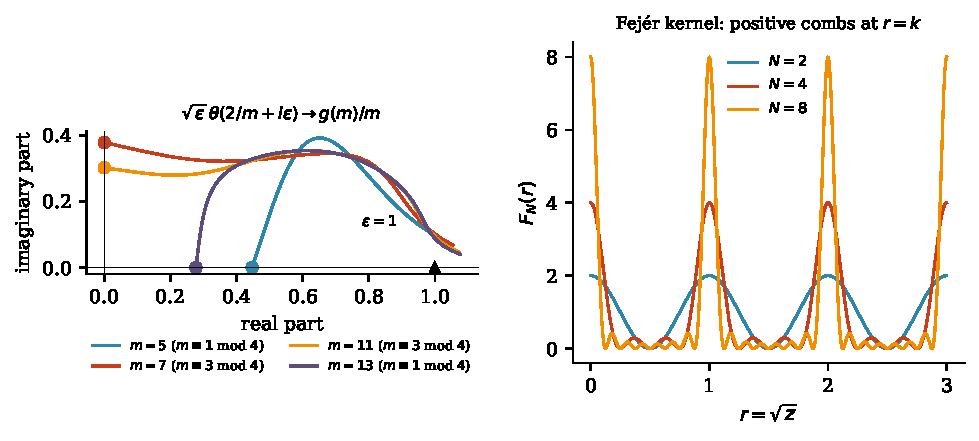
\includegraphics[width=\textwidth]{figs/recip_gauss.pdf}
\caption{Left: Theorem~\ref{thm:recipls} as a Brownian limit. The curves $\varepsilon\mapsto\sqrt\varepsilon\,\theta(2/m+i\varepsilon)$ for $m=5,7,11,13$, $10^{-5}\le\varepsilon\le1$, start near $1$ (triangle) and end at $g(m)/m$, which is real for $m\equiv1\bmod4$ and imaginary for $m\equiv3\bmod4$ (Corollary~\ref{cor:recipgausssign}). Right: the Fej\'er kernel $F_N(r)=\sin^2(\pi Nr)/(N\sin^2\pi r)$ for $N=2,4,8$, the positive combination of winding number cosines in Proposition~\ref{prop:recipfejer}; as $N$ grows it concentrates at the integers $r=k$, that is at the eigenvalues $z=k^2$.}\label{fig:recipgauss}
\end{figure}

The same lemma gives the functional equation of the $L$ function of every even primitive Dirichlet character (stated in Chapter~\ref{ch:02}), with its root number.

\begin{theorem}[the Dirichlet functional equation as a kernel symmetry]\label{thm:recipdirichlet}
Let $\chi$ be a primitive even character modulo $q>1$, $g(\chi)=\sum_{m\bmod q}\chi(m)e^{2\pi im/q}$ its Gauss sum, and $\theta_\chi(t)=\sum_{n\in\Z}\chi(n)e^{-\pi n^2t/q}$ for $t>0$. Then $\theta_\chi(1/t)=\frac{g(\chi)}{\sqrt q}\sqrt t\,\theta_{\bar\chi}(t)$. Equivalently, the P\'olya kernel $\Phi_\chi(u)=\theta_\chi(e^{2u})e^{u/2}$, which satisfies $\Lambda(\frac12+z,\chi)=\int\Phi_\chi(u)e^{zu}du$ for every complex $z$, where $\Lambda(s,\chi)=(q/\pi)^{s/2}\Gamma(s/2)L(s,\chi)$, obeys $\Phi_\chi(-u)=\frac{g(\chi)}{\sqrt q}\Phi_{\bar\chi}(u)$; that is, $\Lambda(s,\chi)=\frac{g(\chi)}{\sqrt q}\Lambda(1-s,\bar\chi)$.
\end{theorem}

\begin{proof}
Primitivity gives $\chi(n)=g(\bar\chi)^{-1}\sum_{m\bmod q}\bar\chi(m)e^{2\pi imn/q}$ for all $n$. Insert this into $\theta_\chi(t)$ and apply Lemma~\ref{lem:recipwrap} with $x=\pi t/q$ and $y=2\pi m/q$. The exponent becomes $(y+2\pi k)^2/(4x)=\pi(m+kq)^2/(qt)$, and $\ell=m+kq$ runs over the class of $m$, so $\theta_\chi(t)=g(\bar\chi)^{-1}\sqrt{q/t}\,\theta_{\bar\chi}(1/t)$. Since $g(\chi)g(\bar\chi)=\chi(-1)q=q$, this is the claim with $t$ and $1/t$ exchanged. The Mellin formula $\int_0^\infty e^{-\pi n^2t/q}t^{s/2}dt/t=\Gamma(s/2)(q/\pi n^2)^{s/2}$ gives $\Lambda(s,\chi)=\frac12\int_0^\infty\theta_\chi(t)t^{s/2}dt/t$, and $t=e^{2u}$ gives the kernel form.
\end{proof}

For a real even primitive $\chi$ the root number $g(\chi)/\sqrt q$ is $\pm1$, since $g(\chi)^2=q$. Whether the P\'olya kernel is even or odd is therefore a sign problem, and for $\chi=(\frac\cdot q)$ with $q\equiv1\bmod4$ prime, $g(\chi)=g(q)=\sqrt q$ by Corollary~\ref{cor:recipgausssign}. So \emph{for primes $q\equiv1\bmod4$, Gauss's sign theorem is the statement that a P\'olya kernel is even}, the $\GL_1$ analogue of Proposition~\ref{prop:recipsym}, and the Brownian limit of Figure~\ref{fig:recipgauss} decides it.

\subsection{The swap for the circle}

The theta transformation can also be proved by a positivity argument, with the Laplace pair of the $2\sin^2$ lemma (compare Section~\ref{sec:recipswap}). Write $\cos u\sqrt z=1-2\sin^2(u\sqrt z/2)$ in \eqref{eq:10dpair} with $a=u^2/4$; since $\int_0^\infty e^{-xz}(\pi z)^{-1/2}dz=x^{-1/2}$ this gives
\begin{equation}\label{eq:recipcospair}
\sqrt{\frac\pi x}\,e^{-u^2/(4x)}=\int_0^\infty e^{-xz}\cos(u\sqrt z)\,\frac{dz}{\sqrt z} .
\end{equation}
The circle $\R/2\pi\Z$ has Laplace eigenvalues $k^2$, $k\in\Z$, playing the part of the $\gamma^2$, and closed geodesics of lengths $2\pi|n|$, playing the part of the prime powers. Its heat trace is $\sum_ke^{-xk^2}$, the Laplace transform of the comb $\sum_{k\in\Z}\delta_{k^2}$, which is the local Thorin comb $\tau_{0,2\pi}$ of Theorem~\ref{thm:10clocal} in its degenerate case $\theta=0$ (Exercise~\ref{ex:10cdegenerate}); \eqref{eq:recipcospair} with $u=2\pi n$ attaches to each winding number $n$ the cosine density $\cos(2\pi n\sqrt z)z^{-1/2}$, a Fourier mode of this comb. In the same way the explicit formula attaches to each prime power $p^m$ a multiple of the cosine density $\cos(m\sqrt z\log p)z^{-1/2}$ (Proposition~\ref{prop:reciprigid}), which by Proposition~\ref{prop:10cdictionary} is, up to sign and the factor $p^{-m/2}$, the $m$th Fourier mode of the local Thorin comb of $p$.

\begin{proposition}[Fej\'er positivity for the circle]\label{prop:recipfejer}\index{Fej\'er kernel}
For $N\ge1$ and $x>0$ let $\mathcal W_N(x)=\sqrt{\pi/x}\sum_{|n|<N}(1-|n|/N)e^{-\pi^2n^2/x}$. Then
\[
\mathcal W_N(x)=\int_0^\infty e^{-xz}F_N(\sqrt z)\frac{dz}{\sqrt z},\qquad F_N(r)=\sum_{|n|<N}\Bigl(1-\frac{|n|}N\Bigr)\cos2\pi nr ,
\]
where $F_N(r)=\sin^2(\pi Nr)/(N\sin^2\pi r)\ge0$ is Fej\'er's kernel, so every $\mathcal W_N$ is completely monotone. As $N\to\infty$ the measures $F_N(\sqrt z)z^{-1/2}dz$ converge vaguely to the comb $\sum_{k\in\Z}\delta_{k^2}=\delta_0+2\sum_{k\ge1}\delta_{k^2}$, and consequently $\sqrt{\pi/x}\sum_ne^{-\pi^2n^2/x}=\sum_ke^{-xk^2}$.
\end{proposition}

\begin{proof}
The integral formula is \eqref{eq:recipcospair} summed with the Fej\'er weights, and the closed form of $F_N$ is classical. In the variable $r=\sqrt z$ the measure is $2F_N(r)dr$ on $[0,\infty)$. The Fej\'er kernel is $1$ periodic, nonnegative, of mass $1$ over a period, and tends to zero uniformly away from the integers; so $2F_N(r)dr$ converges vaguely to $2\sum_{k\ge1}\delta_k+\delta_0$, the half mass at $0$ coming from the half bump on $[0,\frac12]$. The tails are uniformly small, since $\int_{r>R}e^{-xr^2}2F_N(r)dr\le2\sum_{k\ge\lfloor R\rfloor}e^{-xk^2}$, so the Laplace transforms converge: $\mathcal W_N(x)\to1+2\sum_{k\ge1}e^{-xk^2}$. The left side converges to $\sqrt{\pi/x}\sum_ne^{-\pi^2n^2/x}$ by dominated convergence.
\end{proof}

In the variable $r=\sqrt z$, \eqref{eq:recipcospair} is again the normal characteristic function, and the proof is Fej\'er's proof of Poisson summation written as a Laplace transform; it proves Theorem~\ref{thm:reciptheta}, hence Corollaries~\ref{cor:recipgausssign} and \ref{cor:recipqr}, a second time. Its shape is that of Theorem~\ref{thm:recipcm}: the geodesic side, summed with positive weights, is the Laplace transform of a positive measure, which turns out to be the spectral measure. For the circle positivity is free, because the Fej\'er kernel is a square. For an $L$ function the prime powers enter with the signed weights $-\Lambda_\rho(n)n^{-1/2}$ of Definition~\ref{def:recipheat}, and the archimedean term is not positive either: its density $\log N_\rho+2\operatorname{Re}\frac{\gamma'}{\gamma}(\frac12+it,\rho)$ is smallest at $t=0$, where it is negative for $\zeta$, $\Delta$ and the Artin representation of conductor $23$. A Fej\'er type positive summation of the right side of Definition~\ref{def:recipheat} would prove, through Theorem~\ref{thm:recipcm}, holomorphy and GRH at once (Open Problem~\ref{op:recipfejer}).

\subsection{Heat flow and generalized Gauss sums}

For integers $a,c\ge1$ with $ac$ even and $k\in\Z$ put
\[
S(a,c;k)=\sum_{r\bmod c}e^{\pi i(ar^2+2kr)/c},
\]
so that $S(a,c;0)$ is the Gauss sum of Theorem~\ref{thm:recipls}. For $\varepsilon>0$ let $X_\varepsilon$ be the discrete Gaussian, $\Prob(X_\varepsilon=n)=e^{-\pi\varepsilon n^2}/\theta(i\varepsilon)$.

\begin{theorem}[heat flow reciprocity]\label{thm:recipheat}
Let $u=e^{-\pi/(c^2\varepsilon)}$.
\begin{enumerate}
\item[(i)] For every $r$,
\[
\Prob(X_\varepsilon\equiv r\bmod c)=\frac{\sum_ke^{-\pi k^2/(c^2\varepsilon)}e^{2\pi ikr/c}}{c\sum_ke^{-\pi k^2/\varepsilon}},
\]
and the total variation distance from the uniform law on $\Z/c\Z$ is at most $2u/(1-u)$.
\item[(ii)] $\bigl|\E e^{\pi iaX_\varepsilon^2/c}-S(a,c;0)/c\bigr|\le4u/(1-u)$.
\item[(iii)] With $\tau=a/c+i\varepsilon$ and $\kappa=c\varepsilon/a$, for every $\varepsilon>0$,
\[
\begin{split}
&\sqrt{\tau/i}\,\sum_{k\in\Z}e^{-\pi k^2/(c^2\varepsilon)}S(a,c;k)\\
&\qquad=\sqrt{1+i\kappa}\,\sum_{k\in\Z}e^{-\pi k^2(1+i\kappa)/(c^2\varepsilon)}\,\overline{S(c,a;k)} .
\end{split}
\]
\item[(iv)] Consequently, for every $k$,
\[
S(a,c;k)=\sqrt{c/a}\;e^{\pi i/4}\,e^{-\pi ik^2/(ac)}\,\overline{S(c,a;k)}.
\]
\end{enumerate}
\end{theorem}

\begin{proof}
(i) Group $n$ by residue and apply Lemma~\ref{lem:recipwrap} (Poisson summation) to
\[
\sum_me^{-\pi\varepsilon(r+mc)^2}=(c\sqrt\varepsilon)^{-1}\sum_ke^{-\pi k^2/(c^2\varepsilon)}e^{2\pi ikr/c},
\]
and to the normaliser $\theta(i\varepsilon)=\varepsilon^{-1/2}\sum_ke^{-\pi k^2/\varepsilon}$. The difference from $1/c$ is at most
\[
c^{-1}\Bigl(2\sum_{k\ge1}u^{k^2}+2\sum_{k\ge1}e^{-\pi k^2/\varepsilon}\Bigr)\le4c^{-1}\sum_{k\ge1}u^{k^2}
\]
since the denominator is at least $1$, and summing over $r$ and halving gives the bound. (ii) $|e^{\pi iar^2/c}|=1$ and $e^{\pi iar^2/c}$ depends only on $r\bmod c$, so the difference is at most twice the total variation distance. (iii) As in (i), $\sqrt\varepsilon\,\theta(\tau)=c^{-1}\sum_ke^{-\pi k^2/(c^2\varepsilon)}S(a,c;k)$. On the other side $-1/\tau=-c/a+i\delta/(1+i\kappa)$ with $\delta=c^2\varepsilon/a^2$, and Poisson summation with the complex Gaussian weights $e^{-\pi\delta(r+ma)^2/(1+i\kappa)}$ (Lemma~\ref{lem:recipwrap} continued analytically to $\operatorname{Re}x>0$, both sides being holomorphic in $x$) gives
\[
\theta(-1/\tau)=\frac{\sqrt{1+i\kappa}}{c\sqrt\varepsilon}\sum_ke^{-\pi k^2(1+i\kappa)/(c^2\varepsilon)}\overline{S(c,a;-k)}.
\] The theta transformation $\theta(-1/\tau)=\sqrt{\tau/i}\,\theta(\tau)$ and $S(c,a;-k)=S(c,a;k)$ give (iii). (iv) Since $\tau=(a/c)(1+i\kappa)$ and $\kappa/(c^2\varepsilon)=1/(ac)$, (iii) reads
\[
\sum_kw_k\Bigl[\sqrt{a/c}\,e^{-\pi i/4}S(a,c;k)-e^{-\pi ik^2/(ac)}\overline{S(c,a;k)}\Bigr]=0
\]
with $w_k=e^{-\pi k^2/(c^2\varepsilon)}$, for every $\varepsilon>0$. The terms for $k$ and $-k$ coincide, and the functions $\varepsilon\mapsto e^{-\pi k^2/(c^2\varepsilon)}$, $k\ge0$, are Laplace transforms in $1/\varepsilon$ of distinct point masses, so letting $1/\varepsilon\to\infty$ and peeling off the terms one exponent $k^2$ at a time, using that the brackets are bounded, shows that every bracket vanishes.
\end{proof}

Part (iv) is the reciprocity law for generalized quadratic Gauss sums with even linear term (Berndt, Evans and Williams \cite{bew1998}, Theorem~1.2.2). The proof shows that the whole family is a single identity, (iii), between two Gaussian mixtures, which the theta transformation and uniqueness of Laplace transforms separate into its components. At $\varepsilon\downarrow0$ only $k=0$ survives and (iii) becomes the reciprocity of Schaar and Landsberg. Part (i) quantifies the Brownian limit of Theorem~\ref{thm:recipls}: the residue of a discrete Gaussian is uniform up to $e^{-\pi/(c^2\varepsilon)}$ (Figure~\ref{fig:recipzero}, right: for the plotted $c=5$, $7$ and $12$, wherever the bound is below $0.1$ it exceeds the distance by a factor between $3$ and $3.4$). Numerically, (iii) holds to $3\cdot10^{-40}$ at forty digit precision for the four parameter sets tested, and (iv) to $10^{-47}$ at fifty digit precision for all $a,c\le24$ with $ac$ even and $|k|\le6$.

\section{Reciprocity as an identity between random variables}\label{sec:reciplaw}

This section restates reciprocity and its first consequences in the language of probability. The analytic inputs are classical (Brauer's induction theorem, Hecke $L$ functions, the Rankin Selberg method); granted them, the proofs are short and show which part of each statement is probability and which is arithmetic.

\subsection{The Frobenius probability space}

Fix a finite set $S$ of primes and $\sigma>1$. Let $\Omega_S$ be the set of prime powers $p^m$ with $p\notin S$, $m\ge1$, and let $\Prob_\sigma$, Dirichlet's measure, be the probability measure
\[
\Prob_\sigma(\{p^m\})=\frac{p^{-m\sigma}}{m\,Z_\sigma},\qquad Z_\sigma=\sum_{p\notin S,\,m\ge1}\frac{p^{-m\sigma}}m=\log\zeta^S(\sigma)=\log\frac1{\sigma-1}+O(1),
\]
where $\zeta^S$, like $L^S$ below, omits the Euler factors at $S$, and $O(1)$ refers to $\sigma\downarrow1$. A Galois representation $\rho$ as in Section~\ref{sec:recipproblem}, unramified outside $S$ and in the unitary normalisation, so that its Frobenius eigenvalues have absolute value $1$, defines the random variable $a_\rho(p^m)=\tr\rho(\Frob_p^m)$, and when $\rho$ factors through a finite group $G=\Gal(K/\Q)$ it defines the random conjugacy class $F(p^m)=\Frob_p^m$ of $G$. A unitary cuspidal automorphic representation $\pi$ of $\GL_n(\A_\Q)$ unramified outside $S$, with Satake parameters $\{\alpha_{1,p},\dots,\alpha_{n,p}\}$, defines $a_\pi(p^m)=\sum_i\alpha_{i,p}^m$. The definitions are made so that
\begin{equation}\label{eq:reciplogL}
\E_\sigma\bigl[a\,\bar b\,\bigr]=\frac1{Z_\sigma}\log L^S(\sigma,\,\cdot\,)
\end{equation}
for the Rankin Selberg $L$ function of the pair: $L^S(\sigma,\rho\otimes\check\rho')$ for two Galois representations, $L^S(\sigma,\pi\times\tilde\pi')$ for two automorphic ones, the logarithm being the one given by the Dirichlet series. This uses $\overline{\tr\rho'(\Frob_p^m)}=\tr\check\rho'(\Frob_p^m)$ and, for unitary $\pi'$, that the Satake parameters of $\tilde\pi'$ are the conjugates of those of $\pi'$. For $\pi\times\tilde\pi$ the coefficients $|a_\pi(p^m)|^2$ are nonnegative and the series converges for $\sigma>1$ by Jacquet and Shalika \cite{jacquetshalika1981} (Theorem~\ref{thm:ch09rs}); Cauchy Schwarz then gives absolute convergence for every pair. In particular all these variables are square integrable under $\Prob_\sigma$.

\begin{proposition}[reciprocity is almost sure equality]\label{prop:recipas}
Let $\rho$ be an $n$ dimensional Galois representation and $\pi$ a cuspidal automorphic representation of $\GL_n(\A_\Q)$, both unramified outside $S$. Then $L(s,\rho_p)=L(s,\pi_p)$ for all $p\notin S$ if and only if $a_\rho=a_\pi$ $\Prob_\sigma$ almost surely, for one and then every $\sigma>1$.
\end{proposition}

\begin{proof}
$\Prob_\sigma$ charges every point of $\Omega_S$, so almost sure equality is equality at every $p^m$. The power sums $a(p^m)$, $m\ge1$, of $n$ numbers determine their elementary symmetric functions by Newton's identities, hence the characteristic polynomial of $\rho(\Frob_p)$ and the multiset of Satake parameters, hence the local factor; the converse is immediate.
\end{proof}

So Conjecture~\ref{conj:recip}, weakened to agreement at the primes outside a set $S$ containing those where $\rho$ ramifies, is an existence statement about random variables on $(\Omega_S,\Prob_\sigma)$: every Frobenius trace variable $a_\rho$ of an irreducible $\rho$ is almost surely equal to a Hecke eigenvalue variable $a_\pi$ of a cuspidal $\pi$.

\subsection{Chebotarev as convergence in law}

Everything on the Galois side rests on one lemma about Artin $L$ functions of virtual characters, a consequence of Brauer's induction theorem (Section~\ref{sec:ch3artin}).

\begin{lemma}\label{lem:recipvirtual}
Let $K/\Q$ be finite Galois with group $G$, unramified outside $S$, let $\psi$ be a virtual character of $G$, and let $e=\langle\psi,\mathsf{1}\rangle_G$. Then $(s-1)^eL(s,\psi)$ is holomorphic and nonzero near $s=1$, and $\log L^S(\sigma,\psi)=e\log\frac1{\sigma-1}+O(1)$ as $\sigma\downarrow1$.
\end{lemma}

\begin{proof}
By Brauer $\psi=\sum_in_i\operatorname{Ind}_{H_i}^G\chi_i$ with one dimensional $\chi_i$, so $L(s,\psi)=\prod_iL(s,\chi_i)^{n_i}$ with Hecke $L$ functions, each holomorphic and nonzero at $s=1$ except for a simple pole when $\chi_i$ is trivial. The order of the pole is $\sum_in_i\langle\chi_i,\mathsf{1}\rangle_{H_i}$, which is $\langle\psi,\mathsf{1}\rangle_G$ by Frobenius reciprocity. Removing finitely many Euler factors changes nothing near $1$, and the logarithm defined by the Dirichlet series is a continuous branch on $(1,2]$, so it differs from $e\log\frac1{\sigma-1}$ by the logarithm of a continuous nonvanishing function with a limit at $1$.
\end{proof}

\begin{theorem}[Chebotarev in law \cite{chebotarev1926} and the Frobenius distance]\label{thm:recipcheb}\index{Chebotarev density theorem}\index{Frobenius distance}
Let $K/\Q$ be finite Galois with group $G$, unramified outside $S$. Under $\Prob_\sigma$ the random class $F$ converges in law, as $\sigma\downarrow1$, to the image of Haar measure $\mu_G$ on conjugacy classes. Consequently, for Artin representations $\rho,\rho'$ factoring through $G$,
\begin{gather*}
\E_\sigma\bigl[a_\rho\overline{a_{\rho'}}\bigr]\to\langle\chi_\rho,\chi_{\rho'}\rangle_G,\\
d(\rho,\rho')^2:=\lim_{\sigma\downarrow1}\E_\sigma|a_\rho - a_{\rho'}|^2=\int_G|\chi_\rho - \chi_{\rho'}|^2\,d\mu_G .
\end{gather*}
In particular $d(\rho,\rho')=0$ if and only if $\rho\cong\rho'$, and $d(\rho,\rho')^2=2$ for nonisomorphic irreducible $\rho,\rho'$.
\end{theorem}

\begin{proof}
By \eqref{eq:reciplogL} and Lemma~\ref{lem:recipvirtual}, $\E_\sigma\chi(F)=\log L^S(\sigma,\chi)/Z_\sigma\to\langle\chi,\mathsf{1}\rangle_G=\int\chi\,d\mu_G$ for every irreducible character $\chi$. Irreducible characters span the class functions, so $\Prob_\sigma(F\in C)\to|C|/|G|$ for every class $C$, which is convergence in law on the finite set of classes. The remaining statements apply this to the class functions $\chi_\rho\overline{\chi_{\rho'}}$ and $|\chi_\rho-\chi_{\rho'}|^2$, and use that a representation is determined by its character and that irreducible characters are orthonormal.
\end{proof}

The theorem is the Dirichlet density form of Chebotarev's theorem \cite{chebotarev1926}, with the standard proof through Artin $L$ functions rather than Chebotarev's own (Section~\ref{sec:ch3cheb}); the natural density form is Corollary~\ref{cor:ch3cheb}. Only the language is new, and it is worth having for three reasons. First, $d$ is a pseudometric, and by the theorem a metric on isomorphism classes of Artin representations: $\|f\|_\sigma=(\E_\sigma|f|^2)^{1/2}$ is a seminorm, so Minkowski's inequality gives the triangle inequality for $d$ (with $\limsup$ in place of $\lim$ when the limit is not known to exist). Second, the theorem is a statement about couplings: for Artin representations $\rho:G\to\GL_n$, $\rho':G'\to\GL_{n'}$ the pair $(F,F')$ of Frobenius classes lives on one space, and Theorem~\ref{thm:recipcheb} applied to the compositum says that it converges in law to the image of Haar measure of the fibre product $H=\Gal(KK'/\Q)$, embedded in $G\times G'$ by restriction. Third, the theorem separates two levels of information that are easily confused: the \emph{marginal} law of $a_\rho$ (the Sato Tate law of $\rho$, the image of $\mu_G$ under $\chi_\rho$), and the \emph{joint} law of $(a_\rho,a_{\rho'})$.

Marginal laws cannot detect reciprocity (Proposition~\ref{prop:01limits}), but joint laws see more: the limiting joint law of $(a_\rho,a_{\rho'})$ separates nonisomorphic Artin representations with the same marginal law, and at each fixed $\sigma$ reciprocity says that the joint law of $(a_\rho,a_\pi)$ is carried by the diagonal (Proposition~\ref{prop:recipas}). Take $\rho$ the $S_3$ representation of $x^3-x-1$ and $\rho_{31}$ the $S_3$ representation of $x^3+x+1$, of conductor $31$. Their limiting marginal laws are identical (compare Example~\ref{ex:ch3cubic}): $a=2,0,-1$ with probabilities $\frac16,\frac12,\frac13$. The splitting fields are linearly disjoint, since their quadratic subfields $\Q(\sqrt{-23})$ and $\Q(\sqrt{-31})$ differ, so $H=S_3\times S_3$, the coupling is the independent one, and $d(\rho,\rho_{31})^2=2$. Over the $78496$ primes below $10^6$ other than $23$ and $31$ the empirical joint law of $(a_\rho(p),a_{\rho_{31}}(p))$ agrees with the product law $\frac1{36},\frac1{12},\dots,\frac19$ to within $0.0007$ in every cell.

\subsection{Cuspidal orthonormality on the automorphic side}

The automorphic analogue of Theorem~\ref{thm:recipcheb} is the Rankin Selberg method.

\begin{theorem}[orthonormality of cuspidal representations \cite{jpss1983,jacquetshalika1981,moeglinwaldspurger1989,shahidi1981}]\label{thm:recipcusp}
Let $\pi,\pi'$ be unitary cuspidal automorphic representations of $\GL_n(\A_\Q)$ and $\GL_{n'}(\A_\Q)$, unramified outside $S$. Then $\E_\sigma[a_\pi\overline{a_{\pi'}}]\to\delta_{\pi\cong\pi'}$ as $\sigma\downarrow1$. Hence $d(\pi,\pi')^2=2$ when $\pi\not\cong\pi'$, and $d(\pi,\pi')=0$ forces $\pi\cong\pi'$.
\end{theorem}

\begin{proof}
By Jacquet, Piatetski Shapiro and Shalika for $n\ne n'$, and by Jacquet and Shalika and Moeglin and Waldspurger for $n=n'$, $L(s,\pi\times\tilde\pi')$ is holomorphic at $s=1$ unless $\pi'\cong\pi$, when it has a simple pole, and by Shahidi it does not vanish on $\operatorname{Re}s=1$. The argument of Lemma~\ref{lem:recipvirtual} gives $\log L^S(\sigma,\pi\times\tilde\pi')=\delta_{\pi\cong\pi'}\log\frac1{\sigma-1}+O(1)$, and \eqref{eq:reciplogL} finishes the proof. For the distance expand $|a_\pi-a_{\pi'}|^2$.
\end{proof}

Theorems~\ref{thm:recipcheb} and \ref{thm:recipcusp} are one statement on two sides:\index{Schur orthogonality} irreducible Artin representations and cuspidal automorphic representations are both orthonormal systems of random variables in the limit $\sigma\downarrow1$, with unit second moment (the exponential law of Theorem~\ref{thm:recipgamma} below). For irreducible $\ell$ adic representations orthonormality is a conjecture of Tate type \cite{tate1965}, on the pole of $L(s,\rho\otimes\check\rho')$ at $s=1$. Strong multiplicity one\index{strong multiplicity one} follows in one line, by the argument of Jacquet and Shalika \cite{jacquetshalika1981}: if the local factors of two cuspidal representations agree outside a finite set of primes, enlarge $S$ to contain it; then $a_\pi=a_{\pi'}$ on $\Omega_S$, so $d(\pi,\pi')=0$ and $\pi\cong\pi'$.

\subsection{Reciprocity in law}

Call $\rho$ and $\pi$ \emph{reciprocal in law}\index{reciprocity in law} if $d(\rho,\pi)=0$, that is $\E_\sigma|a_\rho-a_\pi|^2\to0$ as $\sigma\downarrow1$.

\begin{corollary}[this book]\label{cor:reciplaw}
Let $\rho,\rho'$ be Artin representations and $\pi,\pi'$ unitary cuspidal automorphic representations, all unramified outside $S$.
\begin{enumerate}
\item[(i)] If $\rho$ and $\pi$ correspond in the sense of Conjecture~\ref{conj:recip}, they are reciprocal in law.
\item[(ii)] If $\rho$ is reciprocal in law with $\pi$ and with $\pi'$, then $\pi\cong\pi'$. If $\rho$ and $\rho'$ are both reciprocal in law with $\pi$, then $\rho\cong\rho'$.
\item[(iii)] If $\rho$ is reciprocal in law with a cuspidal $\pi$, then $\rho$ is irreducible.
\item[(iv)] If $\rho$ is reciprocal in law with $\pi$, then for every $\epsilon>0$ the primes with $|a_\rho(p)-a_\pi(p)|>\epsilon$ have Dirichlet density zero.
\item[(v)] If $\rho$ is automorphic, corresponding to $\pi_0$ in the sense of Conjecture~\ref{conj:recip}, then $\rho$ is reciprocal in law with $\pi$ only for $\pi\cong\pi_0$.
\end{enumerate}
\end{corollary}

\begin{proof}
(i) is Proposition~\ref{prop:recipas} after enlarging $S$. For (ii), the triangle inequality gives $d(\pi,\pi')\le d(\pi,\rho)+d(\rho,\pi')=0$, and Theorem~\ref{thm:recipcusp} applies; likewise $d(\rho,\rho')=0$ and Theorem~\ref{thm:recipcheb} applies. For (iii), Minkowski gives $|\|a_\rho\|_\sigma-\|a_\pi\|_\sigma|\le\|a_\rho-a_\pi\|_\sigma\to0$, while $\|a_\rho\|_\sigma^2\to\langle\rho,\rho\rangle$ and $\|a_\pi\|_\sigma^2\to1$; so $\langle\rho,\rho\rangle=1$. For (iv), with $E$ the set of such primes, $\sum_{p\in E}p^{-\sigma}/Z_\sigma\le\Prob_\sigma(|a_\rho-a_\pi|>\epsilon)\le\epsilon^{-2}\E_\sigma|a_\rho-a_\pi|^2\to0$ by Chebyshev's inequality. (v) is (i) and (ii).
\end{proof}

The corollary is the probabilistic skeleton of the reciprocity dictionary, each item a Hilbert space inequality from the two orthonormality theorems. The agreement in (iv) is only approximate: exact agreement, even on a set of density one, is open in general, and Open Problem~\ref{op:reciplaw} asks for it at all but finitely many primes. Nor does the corollary give existence, and it cannot: the powers of a set of primes of Dirichlet density zero carry $\Prob_\sigma$ mass $o(1)$, so reciprocity in law, like the laws of Proposition~\ref{prop:01limits}, is blind to bounded changes on such a set, while reciprocity itself is not. Figure~\ref{fig:reciplaw} shows the natural density version $\pi(X)^{-1}\sum_{p\le X}|a(p)-b(p)|^2$ of $d^2$ for six pairs. For $\rho$ and the weight one form $\eta(z)\eta(23z)$, whose coefficients were computed independently from the product expansion, it is exactly $0$ for all $X\le10^6$, a pointwise check of the reciprocity for $\rho$ proved by Hecke (Example~\ref{ex:ch3cubic}). For $\rho$ and the data $a'$ obtained from $a_\rho$ by moving $\Frob_2$ from a three cycle to the identity, as in Section~\ref{sec:recipfaces}, it is $1.1\cdot10^{-4}$ and tends to $0$: in law $a'$ is reciprocal to $\eta(z)\eta(23z)$. Yet no cuspidal representation has the local factors of $a'$ at every prime: it would be at distance $0$ from $\eta(z)\eta(23z)$, hence isomorphic to it by Theorem~\ref{thm:recipcusp}, and the Euler factors at $2$ differ. The P\'olya kernel and the Galois heat trace of the later sections do see this one change (Figures~\ref{fig:recipkernel} and \ref{fig:recipheat}). For the other four pairs, $(\rho,\chi_{-23})$, $(\rho,\rho_{31})$, $(\rho,\Delta)$ and $(\Delta,11a1)$, it is $2.000$, $1.998$, $2.005$ and $2.002$ at $X=10^6$, the value $2$ of two orthonormal vectors; over the same primes the mean squares of $a_\rho$ and of $\tau(p)p^{-11/2}$ are $0.997$ and $0.999$.

\begin{figure}[t]
\centering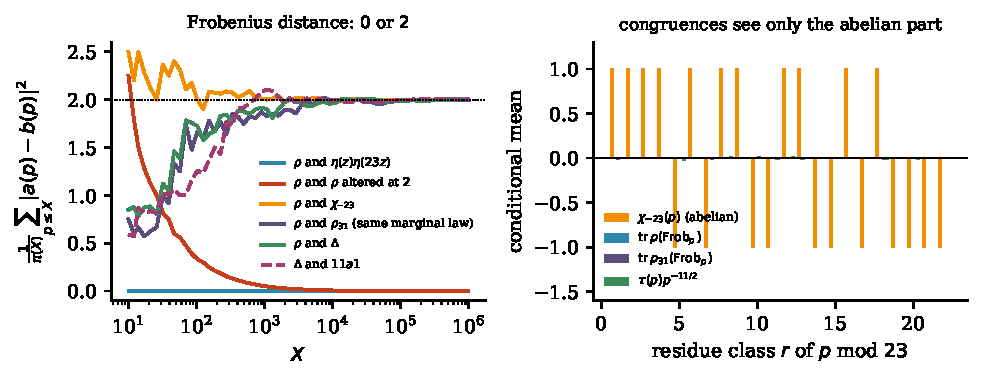
\includegraphics[width=\textwidth]{figs/recip_law.pdf}
\caption{Left: the natural density version $\pi(X)^{-1}\sum_{p\le X}|a(p)-b(p)|^2$ of the squared Frobenius distance. Distinct irreducible or cuspidal objects sit at distance $\sqrt2$ (Theorems~\ref{thm:recipcheb} and \ref{thm:recipcusp}), including $\rho$ and $\rho_{31}$, which have the same marginal law; $\rho$ and $\eta(z)\eta(23z)$ agree at every prime, and $\rho$ altered at $2$ is at distance $0$ from $\rho$ in the limit. Right: means of four Frobenius variables conditional on $p\bmod23$, primes below $10^6$. Only the abelian $\chi_{-23}$ is a function of the residue; the other three are conditionally centred (Proposition~\ref{prop:recipcongruence} for the two Artin traces, Theorem~\ref{thm:recipcusp} with $\pi'$ a Dirichlet character modulo $23$ for $\Delta$).}\label{fig:reciplaw}
\end{figure}

\subsection{Class field theory as measurability}

For $N\ge1$ let $\mathcal F_N$ be the sigma algebra on $\Omega_{S}$ generated by the residue of $p^m$ modulo $N$ (take $S$ to contain the primes dividing $N$). Since $\Frob_p^m$ acts on $\Q(\zeta_N)$ as $\zeta\mapsto\zeta^{p^m}$, $\mathcal F_N$ is generated by the Frobenius class in $\Gal(\Q(\zeta_N)/\Q)$. The conditional law given $\mathcal F_N$ is the probabilistic form of a congruence condition.

\begin{proposition}[congruences see exactly the abelian part; this book, in this form]\label{prop:recipcongruence}\index{Kronecker Weber theorem}
Let $\rho$ be an irreducible Artin representation and $N\ge1$. For every residue $r$ prime to $N$,
\[
\lim_{\sigma\downarrow1}\E_\sigma\bigl[a_\rho\bigm|p^m\equiv r\bmod N\bigr]=\begin{cases}\rho(r)&\text{if }\rho\text{ is inflated from }A_N,\\0&\text{otherwise,}\end{cases}
\]
where $A_N=\Gal(\Q(\zeta_N)/\Q)\cong(\Z/N\Z)^\times$, the first case occurs only when $\dim\rho=1$, and in it $a_\rho$ is itself $\mathcal F_N$ measurable. In particular the Kronecker Weber theorem is equivalent to: every one dimensional Artin representation is $\mathcal F_N$ measurable for some $N$; and no irreducible Artin representation of dimension at least two has a nonzero limiting conditional mean given any congruence.
\end{proposition}

\begin{proof}
Let $K$ be the field cut out by $\rho$ and $\Gamma$ the Galois group of the compositum $L=K(\zeta_N)$, write $A$ for $A_N$, and let $\Gamma_0$ be the subgroup fixing $\Q(\zeta_N)$, so that $A=\Gamma/\Gamma_0$ is abelian. By Theorem~\ref{thm:recipcheb} for $L$, the Frobenius class in $\Gamma$ converges in law to Haar measure, so the conditional mean of $a_\rho$ given that its image in $A$ is $r$ tends to the average of $\chi_\rho$ over the coset $g\Gamma_0$ lying above $r$. Averaging over cosets of $\Gamma_0$ is the orthogonal projection of class functions onto the span of the characters of $A$, so the average equals $\sum_{\psi\in\hat A}\langle\chi_\rho,\psi\rangle_\Gamma\psi(r)$. For irreducible $\rho$ of dimension at least two every $\langle\chi_\rho,\psi\rangle$ vanishes. For one dimensional $\rho$ it is $1$ for $\psi=\rho$ if $\rho$ is inflated from $A$, and $0$ for every $\psi$ otherwise. In the first case $\rho(\Frob_p^m)=\rho(r)$ exactly, which is measurability; here $\rho(r)$ means $\rho$ evaluated at the element $\zeta\mapsto\zeta^r$ of $A_N$.
\end{proof}

This is why reciprocity for $n\ge2$ cannot be a congruence condition, and why it needs automorphic forms: the Hecke eigenvalue $a_\pi(p)$ is the new measurable object that replaces the residue of $p$. Higher conditional moments do see the abelian quotient: for the $S_3$ representation, given $(\frac{p^m}{23})=-1$ the trace is $0$ almost surely, and given $(\frac{p^m}{23})=1$ it is $2$ or $-1$ with limiting conditional probabilities $\frac13,\frac23$, so the limiting conditional mean is $0$ in both cases (Figure~\ref{fig:reciplaw}, right).

\subsection{A dictionary}

\begin{center}\small
\begin{tabular}{p{0.45\textwidth}p{0.45\textwidth}}
\toprule
Arithmetic & Probability\\
\midrule
Frobenius at $p$, Hecke eigenvalue at $p$ & random variables $a_\rho$, $a_\pi$ on $(\Omega_S,\Prob_\sigma)$\\
reciprocity $\rho\leftrightarrow\pi$ & $a_\rho=a_\pi$ almost surely\\
Chebotarev density theorem & convergence in law to Haar measure\\
Schur orthogonality; Rankin Selberg & orthonormality as $\sigma\downarrow1$\\
irreducible Artin; cuspidal & unit second moment; exponential Gamma limit\\
strong multiplicity one & distance zero implies isomorphism\\
class field theory & abelian traces are $\mathcal F_N$ measurable\\
quadratic reciprocity, Gauss's sign & self duality of the normal law\\
functional equation & symmetry of the P\'olya kernel\\
Artin's conjecture and GRH, self dual $\rho$ (Theorem~\ref{thm:recipcm}) & complete monotonicity (Bernstein)\\
converse theorems & a law determined by symmetries of its twists\\
\bottomrule
\end{tabular}
\end{center}

The last line is an analogy rather than a theorem. Twisting by a Dirichlet character is conditioning: since $\mathsf{1}_{p^m\equiv r\bmod N}=\varphi(N)^{-1}\sum_\chi\bar\chi(r)\chi(p^m)$, the twisted series $\sum a(p^m)\chi(p^m)m^{-1}p^{-ms}$ for all $\chi$ modulo $N$ carry the same information as the conditional series given $\mathcal F_N$, and Weil's converse theorem asks for analytic properties of the twists for all moduli in a suitable infinite set, much as the Cram\'er Wold device determines a law on $\R^n$ from its one dimensional projections.

\section{Reciprocity in the Gamma process of a random integer}\label{sec:recipgammaproc}

This section replaces Dirichlet's measure of Section~\ref{sec:reciplaw} by the random integer it comes from, and the random variables by a random measure: label each prime factor of a zeta distributed random integer by its Frobenius class, or by a Satake parameter, and let $\sigma\downarrow1$.

\subsection{The zeta random integer}

For $\sigma>1$ let $N_\sigma=\prod_pp^{e_p}$ be a zeta distributed random integer, $\Prob(N_\sigma=n)=n^{-\sigma}/\zeta(\sigma)$, as in Chapter~\ref{ch:09}, where $e_p$ is written $G_p$. By the compound Poisson form of the geometric law (Exercise~\ref{ex:ch09geometric} of that chapter), $(e_p)_p$ has the law of $(\sum_mmM(p^m))_p$ for independent Poisson variables $M(p^m)$ with means $p^{-m\sigma}/m$, and $\log N_\sigma$ is the zeta subordinator of Proposition~\ref{prop:10dsublaw} at time $1$, with L\'evy measure $\Pi_\sigma$ of Chapter~\ref{ch:10d}.

\begin{lemma}\label{lem:recipzeta}
The exponents $e_p$ are independent and geometric, $\Prob(e_p=k)=(1-p^{-\sigma})p^{-k\sigma}$ for $k\ge0$, and $(\sigma-1)\log N_\sigma$ converges in law to the standard exponential law as $\sigma\downarrow1$.
\end{lemma}

\begin{proof}
The Euler product factorises: for finitely many $t_p$ with $|t_p|\le1$, and $t_p=1$ for the other primes, $\E\prod_pt_p^{e_p}=\zeta(\sigma)^{-1}\prod_p\sum_{k\ge0}t_p^kp^{-k\sigma}=\prod_p(1-p^{-\sigma})/(1-t_pp^{-\sigma})$, a product of geometric generating functions. For the limit, $\E e^{-\lambda(\sigma-1)\log N_\sigma}=\zeta(\sigma+\lambda(\sigma-1))/\zeta(\sigma)\to(1+\lambda)^{-1}$ by the simple pole of $\zeta$ at $1$.
\end{proof}

\subsection{Equidistribution is a Gamma process}

Let $Y$ be a compact metric space, $S$ a finite set of primes, and $(\theta_p)_{p\notin S}$ points of $Y$. We say $(\theta_p)$ is equidistributed with respect to a Borel probability measure $\mu$ on $Y$ if $\pi(t)^{-1}\sum_{p\le t,\,p\notin S}f(\theta_p)\to\int f\,d\mu$ for every continuous $f$. Define the random measure and the marked point process
\[
\Xi_\sigma=\sum_{p\notin S}(\sigma-1)e_p\log p\;\delta_{\theta_p},\qquad \mathcal M_\sigma=\sum_{p\notin S,\,e_p\ge1}\delta_{((\sigma-1)e_p\log p,\;\theta_p)} .
\]
So $\Xi_\sigma$ (a random measure, unrelated to Riemann's $\Xi$ and to the completions $\Xi_\pi$ of Chapter~\ref{ch:10b}) spreads the rescaled logarithm of $N_\sigma$ over the label space, and $\mathcal M_\sigma$ records the rescaled sizes of the prime factors together with their labels. The Gamma random measure $\Gamma_\mu$ with shape measure $\mu$ is the random measure on $Y$ that takes independent values on disjoint Borel sets, with $\Gamma_\mu(B)\sim\mathrm{Gamma}(\mu(B),1)$. Writing $\Gamma_\mu(\lambda)=\int\lambda\,d\Gamma_\mu$, and $\Xi_\sigma(\lambda)$ likewise, its Laplace functional is $\E e^{-\Gamma_\mu(\lambda)}=\exp(-\int\log(1+\lambda)\,d\mu)$ for continuous $\lambda\ge0$, and its atoms form a Poisson process with intensity $x^{-1}e^{-x}dx\,\mu(d\theta)$ \cite{kingman1993}.

\begin{theorem}[equidistribution is a Gamma process; this book]\label{thm:recipgammaproc}
Suppose $(\theta_p)$ is equidistributed with respect to $\mu$. As $\sigma\downarrow1$:
\begin{enumerate}
\item[(i)] $\mathcal M_\sigma$ converges in law, vaguely on $(0,\infty)\times Y$, to the Poisson process with intensity $x^{-1}e^{-x}dx\otimes\mu$: the rescaled sizes of the prime factors of $N_\sigma$ are asymptotically the jumps of a standard Gamma subordinator on $[0,1]$, and their labels are asymptotically independent of the sizes and independent of one another, with law $\mu$;
\item[(ii)] $\Xi_\sigma$ converges in law to $\Gamma_\mu$: for every continuous $\lambda\ge0$ on $Y$, $\E e^{-\Xi_\sigma(\lambda)}\to\exp(-\int_Y\log(1+\lambda)\,d\mu)$.
\end{enumerate}
\end{theorem}

For one point $Y$, part (i) with the sizes normalised by their sum is the Poisson Dirichlet law of the large prime factors of a random integer, due to Billingsley \cite{billingsley1972} for uniform integers; Lloyd \cite{lloyd1984} obtained the limit laws of the largest prime factors of a harmonically distributed integer through the zeta distribution and Poisson variables. Chapter~\ref{ch:pd} develops this: normalised, $\Xi_\sigma$ converges in law to Ferguson's Dirichlet process with base measure $\mu$, and the random integers weighted by the coefficients of the powers of $\zeta$ give the whole Ewens family. The proof of the theorem rests on one estimate.

\begin{lemma}\label{lem:recipnu}
Let $\nu_\sigma=(\sigma-1)\sum_{p\notin S}(\log p)\,p^{-\sigma}\,\delta_{((\sigma-1)\log p,\;\theta_p)}$, a finite measure on $[0,\infty]\times Y$. If $(\theta_p)$ is equidistributed with respect to $\mu$, then $\nu_\sigma$ converges weakly to $e^{-x}dx\otimes\mu$.
\end{lemma}

\begin{proof}
For continuous $f\ge0$ on $Y$ put $A_f(t)=\sum_{p\le t,p\notin S}f(\theta_p)\log p$. Equidistribution and the prime number theorem give $A_f(t)=\mu(f)t+o(t)$ by partial summation, and then the Abelian theorem for Dirichlet series gives
\[
\sum_pf(\theta_p)(\log p)p^{-w}=\frac{\mu(f)}{w-1}+o\Bigl(\frac1{w-1}\Bigr),\qquad w\downarrow1.
\] With $w=\sigma+(\sigma-1)s$, $s\ge0$,
\[
\begin{split}
\int e^{-sx}f(\theta)\,\nu_\sigma(dx,d\theta)&=(\sigma-1)\sum_pf(\theta_p)(\log p)p^{-\sigma-(\sigma-1)s}\\
&\to\frac{\mu(f)}{1+s}=\int_0^\infty e^{-sx}e^{-x}dx\;\mu(f).
\end{split}
\]
By linearity this holds for every continuous $f$. The functions $e^{-sx}f(\theta)$, $s\ge0$, $f\in C(Y)$, span an algebra that contains the constants and separates the points of the compact space $[0,\infty]\times Y$, so it is dense in the continuous functions by Stone and Weierstrass. The total masses converge (take $s=0$, $f=1$), so the convergence extends to all continuous functions.
\end{proof}

\begin{proof}[Proof of Theorem~\ref{thm:recipgammaproc}]
(ii) By Lemma~\ref{lem:recipzeta},
\[
\begin{split}
\log\E e^{-\Xi_\sigma(\lambda)}&=\sum_{p\notin S}\Bigl[\log(1-p^{-\sigma})-\log\bigl(1-p^{-\sigma}e^{-\lambda_pu_p}\bigr)\Bigr]\\
&=-\sum_{p\notin S}p^{-\sigma}\bigl(1-e^{-\lambda_pu_p}\bigr)+R_\sigma ,
\end{split}
\]
where $u_p=(\sigma-1)\log p$, $\lambda_p=\lambda(\theta_p)$ and $R_\sigma=-\sum_{p\notin S}\sum_{m\ge2}m^{-1}p^{-m\sigma}(1-e^{-m\lambda_pu_p})$. Each term of $R_\sigma$ tends to $0$ and is bounded by $p^{-2}$ times a constant, so $R_\sigma\to0$ by dominated convergence. The main term is $-\int h\,d\nu_\sigma$ with $h(x,\theta)=(1-e^{-\lambda(\theta)x})/x$, extended by $\lambda(\theta)$ at $x=0$ and by $0$ at $x=\infty$; $h$ is continuous on $[0,\infty]\times Y$. By Lemma~\ref{lem:recipnu} and Frullani's integral,
\[
\int h\,d\nu_\sigma\to\int_Y\!\int_0^\infty\frac{1-e^{-\lambda(\theta)x}}x\,e^{-x}dx\,\mu(d\theta)=\int_Y\log(1+\lambda)\,d\mu .
\]
(i) Let $F\ge0$ be continuous with compact support in $(0,\infty)\times Y$, say in $[a,b]\times Y$ with $a>0$. Then $-\log\E e^{-\mathcal M_\sigma(F)}=-\sum_p\log(1-y_p)$ with $y_p=\sum_{k\ge1}\Prob(e_p=k)(1-e^{-F(ku_p,\theta_p)})$. The terms with $k\ge2$ contribute at most $\sum_p\sum_{k\ge2}p^{-k}\mathsf{1}\{ku_p\ge a\}$, which tends to $0$ by dominated convergence, and $\sum_py_p^2\to0$ in the same way; replacing $\Prob(e_p=1)$ by $p^{-\sigma}$ costs at most $\sum_pp^{-2}\mathsf{1}\{u_p\ge a\}\to0$, so
\[
-\log\E e^{-\mathcal M_\sigma(F)}=\sum_pp^{-\sigma}(1-e^{-F(u_p,\theta_p)})+o(1)=\int g\,d\nu_\sigma+o(1)
\]
with $g=(1-e^{-F})/x$, which is continuous on $[0,\infty]\times Y$ because $F$ vanishes near $x=0$. Lemma~\ref{lem:recipnu} gives the limit $\int(1-e^{-F})x^{-1}e^{-x}dx\,d\mu$, the Laplace functional of the Poisson process.
\end{proof}

The hypothesis holds for the following label sequences. For a finite Galois extension $K/\Q$ with group $G$, $\theta_p$ is the class $\Frob_p$ in the set $G^\natural$ of conjugacy classes and $\mu=\mu_G$ is the image of Haar measure, by Chebotarev's theorem in its natural density form (Corollary~\ref{cor:ch3cheb}) \cite{chebotarev1926}. For a holomorphic newform of weight $k\ge2$ with trivial character and without complex multiplication, $\theta_p\in[0,\pi]$ is the angle with $x_p=a_p/p^{(k-1)/2}=2\cos\theta_p$, and $\mu$ is the Sato Tate law $\frac2\pi\sin^2\theta\,d\theta$, whose image under $\theta\mapsto2\cos\theta$ is $\ST$, by Theorem~\ref{thm:01satotate} \cite{blght2011}. For two elliptic curves over $\Q$ without complex multiplication and not geometrically isogenous, $\theta_p$ is the pair of angles and $\mu$ the product of two Sato Tate laws, by Theorem~\ref{thm:04joint} \cite{harris2009}.

\begin{corollary}[Chebotarev as a Gamma process; this book]\label{cor:recipchebgamma}
Let $K/\Q$ be finite Galois with group $G$, unramified outside $S$, and for a conjugacy class $C$ let $L_C(\sigma)=(\sigma-1)\sum_{p\notin S,\,\Frob_p\in C}e_p\log p$ be the rescaled part of $\log N_\sigma$ carried by primes with Frobenius in $C$. As $\sigma\downarrow1$:
\begin{enumerate}
\item[(i)] the $L_C(\sigma)$, $C\in G^\natural$, are independent for every $\sigma$, and $L_C(\sigma)$ converges in law to $\mathrm{Gamma}(|C|/|G|,1)$;
\item[(ii)] the shares $L_C/\sum_{C'}L_{C'}$ have a Dirichlet limit law with parameters $(|C|/|G|)_C$, independent of the total, which is standard exponential;
\item[(iii)] for a quadratic character $\chi$, the share of $\log N_\sigma$ carried by the primes with $\chi(p)=-1$ converges to the arcsine law $\pi^{-1}(u(1-u))^{-1/2}du$ on $(0,1)$.
\end{enumerate}
\end{corollary}

\begin{proof}
(i) The $L_C(\sigma)$ depend on disjoint sets of the independent $e_p$, and the limit is Theorem~\ref{thm:recipgammaproc}(ii) on the finite space $G^\natural$, with $\lambda$ a function of the class. (ii) is the beta gamma algebra (independent gamma variables normalised by their sum are Dirichlet and independent of the sum) and the continuous mapping theorem, the total being positive almost surely. (iii) is (ii) for $G=\{\pm1\}$, where the Dirichlet law is $\mathrm{Beta}(\frac12,\frac12)$.
\end{proof}

The mean of the share in (ii) is $|C|/|G|$, which is Chebotarev's density. What the Gamma process adds is the fluctuation: the share does not concentrate, because $\log N_\sigma$ is dominated by a few large prime factors, and their labels are independent Haar samples. In the language of Chapter~\ref{ch:pd}, the limit shares are the masses of the classes under a Dirichlet process with base measure $\mu$, the limit of the normalised labelled factorisation (Theorem~\ref{thm:pddirichlet}). Part (iii) is an arithmetic arcsine law, in the same sense as L\'evy's arcsine law for the time Brownian motion spends positive: a Gamma subordinator split into two halves of equal intensity.

For the $S_3$ field of $x^3-x-1$, ramified only at $23$ (Example~\ref{ex:ch3cubic}; Figure~\ref{fig:ch03_chebotarev} shows its Chebotarev frequencies in natural density), the Laplace transforms $\E e^{-\lambda L_C(\sigma)}$ were computed from the Euler product over the primes below $10^7$, with the remaining primes accounted for by the prime number theorem. Figure~\ref{fig:recipgammaproc}, left, shows them converging to $(1+\lambda)^{-1/6}$, $(1+\lambda)^{-1/2}$ and $(1+\lambda)^{-1/3}$ for the identity class, the transpositions and the three cycles. At $\lambda=1$ the transform differs from its limit by a factor of about $1+\kappa_C(\sigma-1)$, with $\kappa_C$ between $0.38$ and $1.07$ (Theorem~\ref{thm:recipdrift}).

\begin{figure}[t]
\centering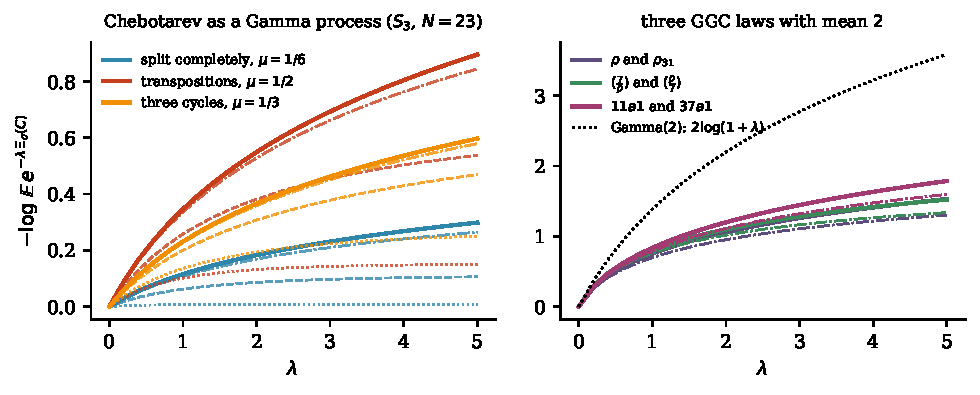
\includegraphics[width=\textwidth]{figs/recip_gammaproc.pdf}
\caption{Left: Corollary~\ref{cor:recipchebgamma} for the $S_3$ field of $x^3-x-1$. Laplace exponents of $L_C(\sigma)=\Xi_\sigma(C)$, from Euler products over $p<10^7$ with a prime number theorem tail, for $\sigma=1.5$ (dotted), $1.1$ (dashed) and $1.01$ (dash dotted) against the Gamma limits $\mu(C)\log(1+\lambda)$. Right: three GGC limits from Theorems~\ref{thm:recipggcfun} and \ref{thm:recipthorin}, all with mean $2$ and with different Thorin measures, against the Gamma$(2)$ limit of the intensity scaling of Theorem~\ref{thm:recipzerotwo}; dash dotted curves are $\sigma=1.01$.}\label{fig:recipgammaproc}
\end{figure}

\subsection{Frobenius functionals are generalized gamma convolutions}

Recall from Definition~\ref{def:ch10ggc} that a GGC is a law on $[0,\infty)$ with Laplace transform
\[
\exp\Bigl(-a\lambda-\int_{(0,\infty)}\log(1+\lambda/t)\,\tau(dt)\Bigr),\qquad\lambda\ge0,
\]
where $a\ge0$ is the drift and $\tau$ the Thorin measure \cite{thorin1977,bondesson1992}. Its mean is $a+\int t^{-1}\,\tau(dt)$, and we call $\tau((0,\infty))$ its Thorin mass. We write $\mathrm{Gamma}(\alpha)$ for the gamma law of shape $\alpha$ and rate $1$, whose Thorin measure is $\alpha\delta_1$, with $\mathrm{Gamma}(0)=\delta_0$.

\begin{theorem}[Frobenius functionals are GGCs; this book]\label{thm:recipggcfun}
Suppose $(\theta_p)$ is equidistributed with respect to $\mu$ and let $Q\ge0$ be continuous on $Y$. Then
\[
\Xi_\sigma(Q)=(\sigma-1)\sum_{p\notin S}e_p\log p\;Q(\theta_p)
\]
converges in law to a GGC with drift zero and Thorin measure $\tau_Q$, the image of $\mu$ restricted to $\{Q>0\}$ under $\theta\mapsto1/Q(\theta)$. Its mean is $\int Q\,d\mu$ and its Thorin mass is $\mu(Q>0)$. Moreover, if $\{Q>0\}$ is a $\mu$ continuity set,
\[
\log\Prob\bigl(\Xi_\sigma(Q)=0\bigr)=-\mu(Q>0)\log\frac1{\sigma-1}+o\Bigl(\log\frac1{\sigma-1}\Bigr).
\]
\end{theorem}

\begin{proof}
Apply Theorem~\ref{thm:recipgammaproc}(ii) to $\lambda Q$: the limit Laplace transform is
\[
\exp\Bigl(-\int\log(1+\lambda Q)\,d\mu\Bigr)=\exp\Bigl(-\int_{\{Q>0\}}\log\bigl(1+\lambda/(1/Q)\bigr)\,d\mu\Bigr),
\]
which is the GGC transform with Thorin measure $\tau_Q$. The mean is $\int t^{-1}\tau_Q(dt)$, which is $\int Q\,d\mu$. For the last statement, $\Xi_\sigma(Q)=0$ exactly when $e_p=0$ for every $p$ with $Q(\theta_p)>0$, so
\[
\log\Prob(\Xi_\sigma(Q)=0)=\sum_{Q(\theta_p)>0}\log(1-p^{-\sigma})=-\sum_{Q(\theta_p)>0}p^{-\sigma}+O(1),
\]
and equidistribution on the continuity set $\{Q>0\}$ gives $\sum_{Q(\theta_p)>0}p^{-\sigma}\sim\mu(Q>0)\log\frac1{\sigma-1}$ by partial summation.
\end{proof}

So the Thorin mass is visible as an exponent, and for Chebotarev labels, where the error term is $O(1)$ by Lemma~\ref{lem:recipvirtual}, the probability that no prime factor of $N_\sigma$ has a label where $Q>0$ is of exact order $(\sigma-1)^{\mu(Q>0)}$. Figure~\ref{fig:recipzero}, left, shows the fitted slopes $0.608$, $0.497$ and $0.989$, against Thorin masses $\frac{11}{18}$, $\frac12$ and $1$ for the three examples of the next section. For $Q=\mathsf 1_C$ Chapter~\ref{ch:pd} computes the constant of this order, and its counterpart for uniform random integers, a case of Serre's theorem on frobenian sets (Theorem~\ref{thm:pdrate}).

\subsection{Reciprocity as vanishing of a Thorin measure}

We now take $Q$ to be a squared discrepancy between two kinds of Frobenius data. The limit is $\delta_0$ exactly when $\tau_Q$ vanishes, so reciprocity laws become vanishing statements, and their failures have computable Thorin measures.

\begin{theorem}[Thorin criteria for reciprocity; this book]\label{thm:recipthorin}
In each case $S$ contains the primes at which the data are ramified (in (b) those ramified in $K(\zeta_N)$, in (c) $2$ and $q$, in (d) the primes of bad reduction of $E$ and $E'$), and $\Xi_\sigma(Q)$ converges in law to the GGC with Thorin measure $\tau_Q$ of Theorem~\ref{thm:recipggcfun}.
\begin{enumerate}
\item[(a)] Artin representations. Let $\rho,\rho'$ be Artin representations unramified outside $S$, with fields $K,K'$ (the fixed fields of their kernels), and put $H=\Gal(KK'/\Q)$ and $Q=|\chi_\rho-\chi_{\rho'}|^2$ on $H^\natural$. Then $\tau_Q$ is the image of Haar probability measure on $\{\chi_\rho\ne\chi_{\rho'}\}\subset H$ under $1/|\chi_\rho-\chi_{\rho'}|^2$. The limit law has mean $\|\chi_\rho-\chi_{\rho'}\|^2_{L^2(H)}$, which is $2$ for nonisomorphic irreducible $\rho,\rho'$, and $\tau_Q=0$ if and only if $\rho\cong\rho'$.
\item[(b)] Abelian reciprocity. Let $\psi$ be a character of finite order of $\Gal(\overline\Q/\Q)$, $\chi$ a Dirichlet character modulo $N$, and $Q=|\psi(\Frob_p)-\chi(p)|^2$. If $\psi\ne\chi$ as characters of $\Gal(K(\zeta_N)/\Q)$, where $K$ is the field of $\psi$, and $\psi\bar\chi$ has order $d$, then
\[
\tau_Q=\frac1d\sum_{j=1}^{d-1}\delta_{1/(4\sin^2(\pi j/d))},
\]
and the limit law has mean $2$ and Thorin mass $1-\frac1d$; otherwise $\tau_Q=0$. The Kronecker Weber theorem is equivalent to the statement that for every $\psi$ there are $N$ and $\chi$ with $\tau_Q=0$.
\item[(c)] Quadratic reciprocity. Let $q\equiv3\bmod4$ be prime. For $Q=|(\frac qp)-(\frac pq)|^2$ the limit law is the gamma law of shape $\frac12$ and rate $\frac14$, that is $2\chi^2_1$, with Thorin measure $\frac12\delta_{1/4}$; for $Q=|(\frac qp)-(\frac pq)(\frac{-1}p)|^2$ the limit is $\delta_0$. For $q\equiv1\bmod4$ the first $Q$ already gives $\delta_0$.
\item[(d)] Elliptic curves. Let $E,E'$ be elliptic curves over $\Q$ without complex multiplication and not geometrically isogenous, with normalised traces $x_p,x'_p$, and $Q=(x_p-x'_p)^2$. Then $\tau_Q$ is the law of $1/(X-X')^2$ for independent $X,X'$ with law $\ST$, so the Thorin mass is $1$ and the limit law has mean $2$. If instead $E'$ is isogenous to $E$, then $Q=0$ for all good $p$ and the limit is $\delta_0$.
\end{enumerate}
\end{theorem}

\begin{proof}
(a) Chebotarev for $KK'$ gives equidistribution of $\Frob_p$ in $H^\natural$ with respect to Haar measure, and Theorem~\ref{thm:recipggcfun} applies with $Y=H^\natural$. The mean is $\int|\chi_\rho-\chi_{\rho'}|^2$; it is $\langle\chi_\rho,\chi_\rho\rangle+\langle\chi_{\rho'},\chi_{\rho'}\rangle-2\operatorname{Re}\langle\chi_\rho,\chi_{\rho'}\rangle=2$ for nonisomorphic irreducibles. Every class of the finite group $H$ has positive Haar measure, so $\tau_Q=0$ forces $\chi_\rho=\chi_{\rho'}$ on $H$, hence $\rho\cong\rho'$.

(b) Here $\psi$ and $\chi$ are both characters of $G_N=\Gal(K(\zeta_N)/\Q)$, $\chi$ through the cyclotomic identification $\Frob_p\mapsto p\bmod N$. Then $Q(g)=|1-(\psi\bar\chi)(g)|^2$. If $\psi\bar\chi$ is nontrivial of order $d$, its values are equidistributed over the $d$th roots of unity under Haar measure on $G_N$, and $|1-e^{2\pi ij/d}|^2=4\sin^2(\pi j/d)$. The mean is $\frac1d\sum_j4\sin^2(\pi j/d)=2$. If $\psi\bar\chi$ is trivial, $Q$ vanishes identically. Kronecker Weber says every $\psi$ factors through some $\Gal(\Q(\zeta_N)/\Q)$, which is the existence of $\chi$ with $\psi=\chi$ on $G_N$; conversely $\tau_Q=0$ gives $\psi=\chi$ on $G_N$.

(c) For odd $p\ne q$, $(\frac qp)$ is the Frobenius character of $\Q(\sqrt q)$, and the law of quadratic reciprocity is $(\frac qp)=(\frac pq)(\frac{-1}p)^{(q-1)/2}$. So for $q\equiv3\bmod4$ the character $\psi\bar\chi$ in (b) is $(\frac{-1}{\cdot})$, of order $d=2$, and $\tau_Q=\frac12\delta_{1/4}$, whose GGC is $(1+4\lambda)^{-1/2}$, the transform of $2\chi^2_1$.

(d) Theorem~\ref{thm:04joint} gives equidistribution of $(x_p,x'_p)$ with respect to $\ST\otimes\ST$, and the diagonal has measure zero, so the mass is $1$; the mean is $\E(X-X')^2=2$. For isogenous curves $a_p=a'_p$ for all good $p$.
\end{proof}

Parts (b) and (c) restate Kronecker Weber and quadratic reciprocity rather than reprove them, since the vanishing of $\tau_Q$ is equivalent to the equality of two characters; what is new is the shape of failure. A mismatched abelian reciprocity is a GGC whose Thorin atoms $1/(4\sin^2(\pi j/d))$ are reciprocals of the squared sines of the $2\sin^2$ lemma (Lemma~\ref{lem:10dsin2}), and omitting the sign factor $(\frac{-1}p)$ from quadratic reciprocity leaves precisely a scaled chi squared variable with one degree of freedom. Numerically (Figure~\ref{fig:recipgammaproc}, right), the three examples $(\rho,\rho_{31})$, $((\frac7p),(\frac p7))$ and $(11a1,37a1)$ all have mean $2$ and different limit laws: orthonormality fixes the mean, and the Thorin measure records the law of the squared discrepancy $Q$, which depends on the joint law of the two kinds of Frobenius data.

\begin{figure}[t]
\centering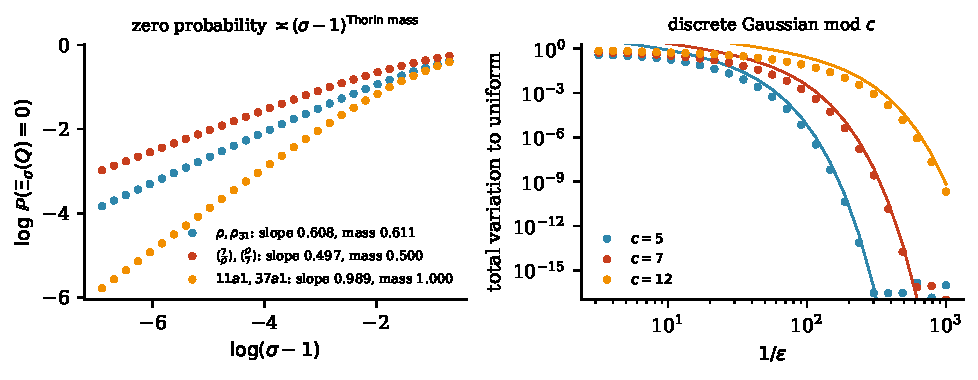
\includegraphics[width=\textwidth]{figs/recip_zeroheat.pdf}
\caption{Left: Theorem~\ref{thm:recipggcfun}. The probability that no prime factor of $N_\sigma$ has a label where $Q>0$, computed from the Euler product over primes below $10^7$ with a prime number theorem tail, decays like $(\sigma-1)^m$, with $m$ the Thorin mass. Right: Theorem~\ref{thm:recipheat}. Total variation distance between a discrete Gaussian with parameter $\varepsilon$ reduced modulo $c$ and the uniform law (dots), against the bound of part (i) (lines). For $c=5$ and $7$ the dots that level off near $10^{-16}$, above the lines, are rounding errors of the double precision computation, not distances.}\label{fig:recipzero}
\end{figure}

\subsection{A second scaling and a zero two law}

Theorem~\ref{thm:recipggcfun} uses $Q$ as a mark on the jumps of a fixed random integer. One can instead let $Q$ change the intensity: take two of the Frobenius variables $a,b$ of Section~\ref{sec:reciplaw} (each an $a_\rho$ or an $a_\pi$, fixed in the next theorem), put $Q_m(p)=|a(p^m)-b(p^m)|^2\ge0$, and replace the zeta integer by the random integer $N_{Q,\sigma}$ with $\Prob(N_{Q,\sigma}=n)\propto d_Q(n)n^{-\sigma}$, where $\sum_nd_Q(n)n^{-s}=D_Q(s)$ is the Dirichlet series with $\log D_Q(s)=\sum_{p\notin S,m}Q_m(p)m^{-1}p^{-ms}$. Its logarithm $X_\sigma=\log N_{Q,\sigma}$ is the discrepancy subordinator; for $b=0$ it is the Rankin Selberg subordinator of Theorem~\ref{thm:recipgamma}, which is the case $\rho'=0$ of the next theorem.

\begin{theorem}[zero two law; this book]\label{thm:recipzerotwo}
(a) For Artin representations $\rho,\rho'$ with $a=\tr\rho$, $b=\tr\rho'$, $(\sigma-1)X_\sigma$ converges in law to $\mathrm{Gamma}(\|\chi_\rho-\chi_{\rho'}\|^2)$, a GGC with Thorin measure $\|\chi_\rho-\chi_{\rho'}\|^2\delta_1$ and integer shape; for irreducible $\rho,\rho'$ the shape is $0$ or $2$.
(b) For unitary cuspidal automorphic representations $\pi,\pi'$ of $\GL_n(\A_\Q)$, $\GL_{n'}(\A_\Q)$ with $a=a_\pi$, $b=a_{\pi'}$, the limit is $\delta_0$ if $\pi\cong\pi'$ and $\mathrm{Gamma}(2)$ otherwise.
\end{theorem}

\begin{proof}
$D_Q=L(\rho\otimes\check\rho)L(\rho'\otimes\check\rho')/(L(\rho\otimes\check\rho')L(\rho'\otimes\check\rho))$ up to finitely many Euler factors, the $L$ function of the virtual character $|\chi_\rho-\chi_{\rho'}|^2$. By Lemma~\ref{lem:recipvirtual} it has a pole of order $e=\langle|\chi_\rho-\chi_{\rho'}|^2,1\rangle=\|\chi_\rho-\chi_{\rho'}\|^2$ at $s=1$ and is otherwise holomorphic and nonzero near $1$, so $\E e^{-\lambda(\sigma-1)X_\sigma}=D_Q(\sigma+\lambda(\sigma-1))/D_Q(\sigma)\to(1+\lambda)^{-e}$. For (b), the same computation with $L(s,\pi\times\tilde\pi')$, which by Jacquet, Shalika, Moeglin, Waldspurger and Shahidi \cite{jacquetshalika1981,moeglinwaldspurger1989,shahidi1981} has a simple pole at $1$ exactly when $\pi'\cong\pi$ and no zero on $\operatorname{Re}s=1$, gives $e=2-2\delta_{\pi\cong\pi'}$.
\end{proof}

The two scalings give two GGCs with the same mean $\int Q\,d\mu$: in Theorem~\ref{thm:recipzerotwo} the Thorin measure $\tau_Q$ of Theorem~\ref{thm:recipggcfun} collapses to a single atom at $1$ carrying the mean. Integrality of the collapsed shape is Schur orthogonality, and the value $2$ for distinct irreducibles is the orthonormality of characters; for cuspidal pairs it is Rankin Selberg. The natural extension to the mixed case is the following conjecture.

\begin{conjecture}[mixed zero two law]\label{conj:recipmixed}
Let $\rho$ be an irreducible Artin representation of dimension $n$ and $\pi$ a unitary cuspidal automorphic representation of $\GL_n(\A_\Q)$, with $a=\tr\rho$ and $b=a_\pi$. Then $(\sigma-1)X_\sigma$ converges in law to $\delta_0$ or to $\mathrm{Gamma}(2)$, and to $\delta_0$ exactly when $L(s,\rho_p)=L(s,\pi_p)$ for almost all $p$.
\end{conjecture}

\begin{proposition}[this book]\label{prop:recipmixed}
(i) If $\rho$ is automorphic, Conjecture~\ref{conj:recipmixed} holds for $\rho$ and every $\pi$. Hence it holds for $n=1$, for odd two dimensional $\rho$, and for two dimensional $\rho$ with solvable image.
(ii) Unconditionally, $\limsup_{\sigma\downarrow1}\E[(\sigma-1)X_\sigma]\le4$ and $\E[((\sigma-1)X_\sigma)^2]$ stays bounded, so under the conjecture $\E[(\sigma-1)X_\sigma]$ tends to $0$ or $2$.
(iii) If the limit is $\delta_0$ then $\rho$ and $\pi$ are reciprocal in law, so $\pi$ is unique up to isomorphism and, for every $\epsilon>0$, $|a_\rho(p)-a_\pi(p)|\le\epsilon$ outside a set of primes of Dirichlet density zero (Corollary~\ref{cor:reciplaw}(ii) and (iv)).
\end{proposition}

\begin{proof}
(i) If $\rho$ corresponds to $\pi_\rho$, then $a=a_{\pi_\rho}$ off a finite set and Theorem~\ref{thm:recipzerotwo}(b) applies to $(\pi_\rho,\pi)$. The listed cases are class field theory, Khare and Wintenberger \cite{kharewintenberger2009,kharewintenberger2009b} with work of Kisin \cite{kisin2009}, and Langlands and Tunnell \cite{langlands1980,tunnell1981}. (ii) The mean is $(\sigma-1)\sum_{p,m}Q_m(p)(\log p)p^{-m\sigma}$. Since $Q_m\le2|a(p^m)|^2+2|b(p^m)|^2$, it is at most $2(\sigma-1)(-L'/L)(\sigma,\rho\otimes\check\rho)+2(\sigma-1)(-L'/L)(\sigma,\pi\times\tilde\pi)$ up to finitely many Euler factors, and both terms tend to $2$ because each $L$ function has a simple pole at $1$. The same bound for $(\log D_Q)''(\sigma)$, the variance of $X_\sigma$, gives $\operatorname{Var}((\sigma-1)X_\sigma)\le4+o(1)$, since $(\sigma-1)^2(\log L)''(\sigma)\to1$ at a simple pole; so $\E[((\sigma-1)X_\sigma)^2]\le20+o(1)$, and the means converge whenever the laws do. (iii) Put
\[
\eta_\sigma=(\sigma-1)\sum_{p,m}Q_m(p)(\log p)p^{-m\sigma}\delta_{(\sigma-1)m\log p}.
\]
The Laplace exponent at $\lambda=1$ is
\[
\int\frac{1-e^{-x}}x\,\eta_\sigma(dx)\ge\frac{1-e^{-K}}K\,\eta_\sigma([0,K]),
\]
so $\eta_\sigma([0,K])\to0$ for every $K$; the tails $\eta_\sigma([K,\infty))$ are at most $4e^{-K}+o(1)$ by the same bound as in (ii) applied to the Gamma limits of $|a|^2$ and $|b|^2$. Hence $(\sigma-1)\sum Q_m(p)(\log p)p^{-m\sigma}\to0$, and integrating in $\sigma$, $\log D_Q(\sigma)=\int_\sigma^2\sum Q_m(p)(\log p)p^{-mw}dw+O(1)=o(\log\frac1{\sigma-1})$, which is the definition of reciprocity in law.
\end{proof}

Conjecture~\ref{conj:recipmixed} follows from reciprocity (Proposition~\ref{prop:recipmixed}(i)) but does not imply it, because it asserts no existence: for a nonautomorphic $\rho$ it predicts the limit $\mathrm{Gamma}(2)$ for every $\pi$. It is the orthogonality half of reciprocity, and existence is the other half: by its last clause, reciprocity for $\rho$ is equivalent to the conjecture together with the existence of one $\pi$ whose limit is $\delta_0$. If $L(s,\rho_p)=L(s,\pi_p)$ for almost all $p$, then $Q_m(p)=0$ outside a finite set of primes and the limit is $\delta_0$ unconditionally; conversely, without the conjecture, a $\delta_0$ limit makes $\rho$ and $\pi$ reciprocal in law (Proposition~\ref{prop:recipmixed}(iii)), and whether that forces $a_\rho(p)=a_\pi(p)$ for all but finitely many $p$ is Open Problem~\ref{op:reciplaw}.

\subsection{Second order Chebotarev: the Euler Kronecker drift}

The Gamma limit of Corollary~\ref{cor:recipchebgamma} is approached at rate $\sigma-1$ (Figure~\ref{fig:recipdrift}), with a constant given by logarithmic derivatives of Artin $L$ functions at $s=1$ and a prime power term.

For a character $\chi$ of $G=\Gal(K/\Q)$ and the finite set $S$ put
\[
\gamma^S(\chi)=\lim_{s\to1}\Bigl(\frac{(L^S)'}{L^S}(s,\chi)+\frac{\delta_{\chi=1}}{s-1}\Bigr),
\]
where $L^S$ omits the Euler factors at $S$. For $\chi\ne1$ this is
\[
\frac{L'}L(1,\chi)+\sum_{p\in S}\sum_{m\ge1}\tr(\Frob_p^m\mid V_\chi^{I_p})\,(\log p)\,p^{-m},
\]
where $V_\chi$ is a representation with character $\chi$ and $I_p$ an inertia group at $p$, and for $\chi=1$ it is $\gamma_{\mathrm E}+\sum_{p\in S}\frac{\log p}{p-1}$ with $\gamma_{\mathrm E}$ Euler's constant. The Euler Kronecker constant of $K$ in Ihara's sense \cite{ihara2006} is
\[
\gamma_K=\lim_{s\to1}\Bigl(\frac{\zeta_K'}{\zeta_K}(s)+\frac1{s-1}\Bigr)=\sum_\chi\chi(1)\gamma^\emptyset(\chi),
\]
and $\gamma_K^S$ denotes the same constant for $\zeta_K$ with the Euler factors above $S$ removed.

\begin{theorem}[Euler Kronecker drift; this book]\label{thm:recipdrift}
Let $K/\Q$ be finite Galois with group $G$, unramified outside $S$, and $C$ a conjugacy class. Uniformly for $\lambda$ in compact subsets of $[0,\infty)$,
\[
\log\E e^{-\lambda L_C(\sigma)}=-\mu(C)\log(1+\lambda)+\kappa_C\,\lambda\,(\sigma-1)+O\bigl((\sigma-1)^2\bigr),
\]
with
\[
\kappa_C=\mu(C)\sum_\chi\overline{\chi(C)}\,\gamma^S(\chi)\;-\;\sum_{p\notin S}\sum_{m\ge2}\bigl[\mathsf 1_C(\Frob_p)-\mathsf 1_C(\Frob_p^m)\bigr]\,(\log p)\,p^{-m},
\]
the sum over irreducible characters. In particular $\E L_C(\sigma)=\mu(C)-\kappa_C(\sigma-1)+O((\sigma-1)^2)$: to first order the Gamma limit is shifted by the deterministic amount $-\kappa_C(\sigma-1)$. For the class of primes that split completely,
\[
\kappa_{\{1\}}=\frac{\gamma_K^S}{|G|}+\sum_{p\notin S,\;\Frob_p\ne1}\;\sum_{m\ge2,\;\Frob_p^m=1}(\log p)\,p^{-m},
\]
the Euler Kronecker constant of $K$ with the Euler factors above $S$ removed, divided by the degree, plus a nonnegative prime power term. For a class function $Q\ge0$, independence of the $L_C(\sigma)$ gives $\log\E e^{-\lambda\Xi_\sigma(Q)}=-\sum_C\mu(C)\log(1+\lambda Q_C)+\kappa_Q\lambda(\sigma-1)+O((\sigma-1)^2)$ with $\kappa_Q=\sum_CQ_C\,\kappa_C$.
\end{theorem}

\begin{proof}
By Lemma~\ref{lem:recipzeta}, $\log\E e^{-\lambda L_C(\sigma)}=P_C(\sigma')-P_C(\sigma)$ with $\sigma'=\sigma+\lambda(\sigma-1)$ and $P_C(s)=\sum_{p\notin S,\Frob_p\in C}\sum_mm^{-1}p^{-ms}$. Expand $\mathsf 1_C=\sum_\chi c_\chi\chi$ with $c_\chi=\mu(C)\overline{\chi(C)}$. Since $\sum_\chi c_\chi\chi(g^m)=\mathsf 1_C(g^m)$,
\[
\sum_\chi c_\chi\log L^S(s,\chi)=\sum_{p\notin S}\sum_m\frac{\mathsf 1_C(\Frob_p^m)}{m\,p^{ms}},
\]
so that
\[
P_C(s)=\sum_\chi c_\chi\log L^S(s,\chi)+R_C(s),
\]
with
\[
R_C(s)=\sum_{p\notin S}\sum_{m\ge2}\bigl[\mathsf 1_C(\Frob_p)-\mathsf 1_C(\Frob_p^m)\bigr]m^{-1}p^{-ms}
\]
holomorphic on $\operatorname{Re}s>\frac12$. By Brauer's theorem each $L^S(s,\chi)$, $\chi\ne1$, is holomorphic and nonzero near $s=1$, and $(s-1)\zeta^S(s)$ is too. So $h_C(s)=P_C(s)-\mu(C)\log\frac1{s-1}$ is real analytic near $s=1$, with $h_C'(1)=\sum_\chi c_\chi\gamma^S(\chi)+R_C'(1)=\kappa_C$. Then $P_C(\sigma')-P_C(\sigma)=-\mu(C)\log(1+\lambda)+h_C(\sigma')-h_C(\sigma)$, and Taylor's theorem gives the expansion. The mean is minus the derivative in $\lambda$ at $0$. For $C=\{1\}$, $c_\chi=\chi(1)/|G|$ and $\sum_\chi\chi(1)\gamma^S(\chi)=\gamma_K^S$ because $\zeta_K^S=\prod_\chi L^S(s,\chi)^{\chi(1)}$; the prime power term is nonnegative because a power of the identity is the identity. The statement for $Q$ follows by summing over classes.
\end{proof}

For the $S_3$ field of $x^3-x-1$ the set $S$ consists of $2$, $7$, $11$, $23$, $31$ and $37$, the primes that are bad for some example of this section. PARI/GP gives $\frac{L'}L(1,\chi_{-23})=-0.42212$ and $\frac{L'}L(1,\rho)=1.01706$, so $\gamma_K=\gamma_{\mathrm E}-0.42212+2(1.01706)=2.18922$; with the Euler factors above $S$ removed, $\gamma_K^S=3.59058$, and the prime power term of Theorem~\ref{thm:recipdrift} is $0.14171$, so $\kappa_{\{1\}}=3.59058/6+0.14171=0.74014$. Theorem~\ref{thm:recipdrift} predicts the drifts in the first row below; the second row is the intercept of a linear fit of $[\log\E e^{-L_C(\sigma)}+\mu(C)\log2]/(\sigma-1)$ over $\sigma-1\in[0.00125,0.04]$ (for $Q$, with $\frac12\log5$ in place of $\mu(C)\log2$), from the Euler products used for Figure~\ref{fig:recipgammaproc} (Figure~\ref{fig:recipdrift}).
\begin{center}\small
\begin{tabular}{lcccc}
\toprule
& identity & transpositions & three cycles & $Q=|(\frac7p)-(\frac p7)|^2$\\
\midrule
$\kappa$ predicted & $0.74014$ & $1.07416$ & $0.37746$ & $4.4189$\\
fitted & $0.73881$ & $1.07365$ & $0.37710$ & $4.4058$\\
\bottomrule
\end{tabular}
\end{center}
The three class drifts add up to $\gamma_{\mathrm E}+\sum_{p\in S}\frac{\log p}{p-1}=2.19176$, the drift of $(\sigma-1)\sum_{p\notin S}e_p\log p$, the part of $(\sigma-1)\log N_\sigma$ carried by the primes outside $S$; for $(\sigma-1)\log N_\sigma$ itself the drift is $\gamma_{\mathrm E}$. The prime power term of $\kappa_C$ is the Dirichlet density counterpart of the prime square bias that Section~\ref{sec:ch3cheb} measures for the same field. For uniform random integers below $x$, with $S$ the set of ramified primes, a size biased prime factor has Frobenius in $C$ with probability $\mu(C)+(\gamma_{\mathrm E}\mu(C)-\kappa_C)/(\log x-1)+O((\log x)^{-2})$ (Theorem~\ref{thm:pdmertens}).

\begin{figure}[t]
\centering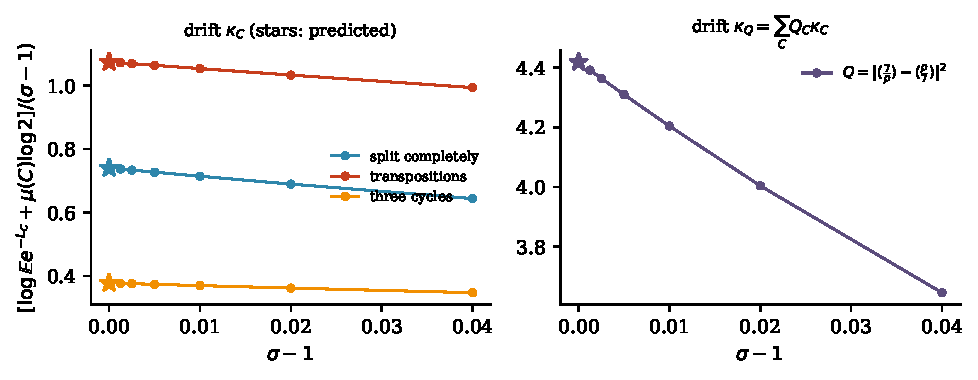
\includegraphics[width=\textwidth]{figs/recip_drift.pdf}
\caption{Theorem~\ref{thm:recipdrift}. The normalised deviation of the logarithm of the Laplace transform from its Gamma limit, at $\lambda=1$, as $\sigma\downarrow1$, for the three classes of the $S_3$ field (left) and for the quadratic reciprocity discrepancy with the sign factor omitted (right). Stars are the predicted drifts.}\label{fig:recipdrift}
\end{figure}

Under GRH Ihara showed that $\gamma_K$ is at most about $2\log\log\sqrt{|d_K|}$ \cite{ihara2006}. Since $(\gamma_K^S-\gamma_K)/|G|\le\sum_{p\in S}\frac{\log p}{p-1}$ and the prime power term is at most $\sum_p\frac{\log p}{p(p-1)}<0.76$, GRH bounds the drift of the split class from above by about $2\log\log\sqrt{|d_K|}/|G|+\sum_{p\in S}\frac{\log p}{p-1}+0.76$. No lower bound of this form holds for all $K$: $\gamma_K$ is negative when $K$ has many primes of small norm, and Ihara's lower bound, which needs no hypothesis, is only of order $-\log\sqrt{|d_K|}$ \cite{ihara2006}. Ihara's bounds say nothing about the other classes, whose drifts involve the individual values $\frac{L'}L(1,\chi)$, not $\gamma_K$ alone.

\section{One function with two faces}\label{sec:recipfaces}

Let $f(z)=\sum_{n\ge1}a_ne^{2\pi inz}$ with $a_n=O(n^{(k-1)/2+\epsilon})$, $k\ge1$ an integer, $N\ge1$, and put $\Lambda(s)=(\sqrt N/2\pi)^s\Gamma(s)\sum a_nn^{-s}$. As in Section~\ref{sec:02mellin}, termwise integration gives, for $\operatorname{Re}s$ large,
\begin{equation}\label{eq:recipmellin}
\begin{gathered}
\Lambda(s)=\int_0^\infty f\Bigl(\frac{iy}{\sqrt N}\Bigr)y^{s}\frac{dy}y,\\
\Lambda\Bigl(\frac k2+t\Bigr)=\int_{\R}\Phi_f(u)e^{tu}\,du,\qquad \Phi_f(u)=f\Bigl(\frac{ie^u}{\sqrt N}\Bigr)e^{ku/2}.
\end{gathered}
\end{equation}
We call $\Phi_f$ the \emph{P\'olya kernel}\index{P\'olya kernel} of the coefficient sequence (for $\Delta$ see Exercise~\ref{ex:recipdelta}); when it is nonnegative and integrable it is, up to normalisation, the density of the P\'olya variable $W_f$ with $\E e^{tW_f}=\Lambda(\frac k2+t)/\Lambda(\frac k2)$. The kernel is built from the coefficients alone: if they are the Dirichlet coefficients of a Galois $L$ function, $\Phi_f$ is a Galois object, and if $f$ is a modular form, $\Phi_f$ is the restriction of an automorphic form to the geodesic $i\R_{>0}$. Reciprocity asks when the two descriptions coincide.

\begin{proposition}[Hecke's criterion as a symmetry; this book]\label{prop:recipsym}
With $f$ and $\Phi_f$ as above and $\varepsilon\in\{\pm1\}$, the following are equivalent.
\begin{enumerate}
\item[(i)] $\Phi_f(-u)=\varepsilon\,\Phi_f(u)$ for all real $u$.
\item[(ii)] $f(-1/(Nz))=\varepsilon\,i^{-k}N^{k/2}z^kf(z)$ for all $z$ in the upper half plane.
\item[(iii)] $\Lambda$ extends to an entire function, bounded in vertical strips, with $\Lambda(k-s)=\varepsilon\Lambda(s)$.
\end{enumerate}
For $N=1$, $k$ even and $\varepsilon=(-1)^{k/2}$ these are equivalent to: $f$ is a cusp form of weight $k$ for $\SL_2(\Z)$.
\end{proposition}

\begin{proof}
Put $y=e^u/\sqrt N$, so that $ie^{-u}/\sqrt N$ is $i/(Ny)$. Then (i) reads
\[
f\bigl(i/(Ny)\bigr)=\varepsilon N^{k/2}y^kf(iy),
\]
which is (ii) on the imaginary axis, since $-1/(N\cdot iy)$ equals $i/(Ny)$ and $z^k=i^ky^k$. Both sides of (ii) are holomorphic in the upper half plane, so agreement on the imaginary axis gives agreement everywhere; this proves (i) if and only if (ii). The equivalence of (ii) and (iii) is Hecke's theorem \cite{hecke1936} (Section~\ref{sec:02mellin}): split \eqref{eq:recipmellin} at $y=1$, the fixed point of the Fricke involution $y\mapsto1/y$ in this variable, and use (ii) to fold the lower range onto the upper one, which gives the continuation, the bound and the functional equation; conversely Mellin inversion and a contour shift recover (ii) from (iii). For $N=1$, the group $\SL_2(\Z)$ is generated by $z\mapsto z+1$, which every $q$ series respects, and $z\mapsto-1/z$, which is (ii) with $\varepsilon i^{-k}=1$; cuspidality follows from $a_0=0$ and the growth of the coefficients.
\end{proof}

So at level one, reciprocity for a Galois representation of conductor $1$ with the Hodge numbers of weight $k$ is the statement that one function on the line, built from its Frobenius traces, is even (odd when $k\equiv2\bmod4$). When the kernel is a density, it says that a random variable built from primes is symmetric. For level $N$ the symmetry (i) is only the Fricke involution; Weil's converse theorem asks for the analogous symmetries of the twisted kernels $\Phi_{f\otimes\chi}$, which pair $\chi$ with $\bar\chi$. Chapter~\ref{ch:flt} reads the modularity of elliptic curves in this form. Chapter~\ref{ch:lap} computes the kernel of $\eta(z)\eta(23z)$, there normalised as $2\Phi_f$, from the Artin $L$ function on the critical line rather than from the $q$ expansion, by Bromwich inversion, which uses the holomorphy that Hecke's theorem supplies (Proposition~\ref{prop:lappolya}).

The symmetry is extremely sensitive to the Frobenius data. Figure~\ref{fig:recipkernel} shows $\Phi_f$ for the weight one form of level $23$ attached to the $S_3$ representation $\rho$ of $x^3-x-1$, and for $\Delta$. With the true Frobenius traces the kernels are symmetric to $2\cdot10^{-16}$ and $2\cdot10^{-18}$. If the Frobenius data at $2$ alone are changed ($\Frob_2$ moved from order three to the identity for $\rho$, the sign of $\tau(2)$ reversed for $\Delta$), and all coefficients $a_n$ are rebuilt multiplicatively, the maximal asymmetry becomes $1.19$ for the Artin representation, whose true kernel has maximum $0.178$, and $1.4\cdot10^{-3}$ for $\Delta$, whose true kernel has maximum $1.8\cdot10^{-3}$.

\begin{figure}[t]
\centering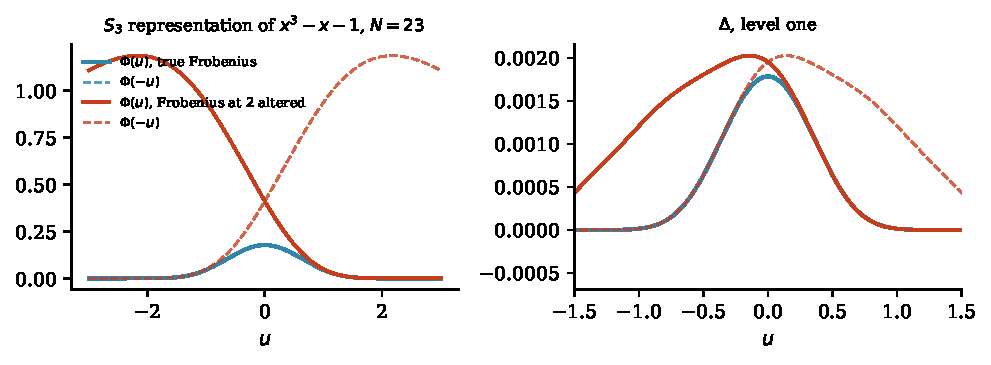
\includegraphics[width=\textwidth]{figs/recip_kernel.pdf}
\caption{Reciprocity as a symmetry. The P\'olya kernel $\Phi_f(u)$ built from Frobenius traces (blue) coincides with $\Phi_f(-u)$ (dashed). Changing the Frobenius data at the single prime $2$ (red) destroys the symmetry. Left: the $S_3$ representation of conductor $23$; right: $\Delta$.}\label{fig:recipkernel}
\end{figure}

\section{The Galois side: Rankin Selberg subordinators}\label{sec:recipgalois}

Infinite divisibility on the Galois side comes for free once one passes to $\rho\otimes\check\rho$. Let $S$ be the set of ramified primes and
\begin{gather*}
D^S(s)=L^S(s,\rho\otimes\check\rho)=\prod_{p\notin S}\det\bigl(1-(\rho\otimes\check\rho)(\Frob_p)p^{-s}\bigr)^{-1},\\
\log D^S(s)=\sum_{p\notin S}\sum_{m\ge1}\frac{|a_\rho(p^m)|^2}{m\,p^{ms}} .
\end{gather*}
All logarithmic coefficients are nonnegative, so for $\sigma>1$ the function $\lambda\mapsto D^S(\sigma+\lambda)/D^S(\sigma)$ is the Laplace transform of a compound Poisson subordinator $X_\sigma$ with L\'evy measure $\sum_{p,m}|a_\rho(p^m)|^2m^{-1}p^{-m\sigma}\delta_{m\log p}$. This is the Galois counterpart of the Rankin Selberg laws of Theorem~\ref{thm:ch09rs} and of the zeta subordinators of Chapter~\ref{ch:10d}.

\begin{theorem}[Gamma shape detects irreducibility; this book]\label{thm:recipgamma}
Let $\rho$ be an Artin representation and $m=\langle\rho,\rho\rangle$ the sum of the squares of the multiplicities of its irreducible constituents. As $\sigma\downarrow1$, $(\sigma-1)X_\sigma$ converges in law to the Gamma law with shape $m$ and scale $1$. In particular $\rho$ is irreducible if and only if the limit is the standard exponential law.
\end{theorem}

\begin{proof}
By Schur's lemma the trivial representation occurs in $\rho\otimes\check\rho=\operatorname{End}(\rho)$ with multiplicity $\langle\rho,\rho\rangle=m$, so by Lemma~\ref{lem:recipvirtual} for $\psi=\rho\otimes\check\rho$ (finitely many Euler factors change nothing near $s=1$), $D^S(s)=(s-1)^{-m}G(s)$ with $G$ holomorphic and nonzero near $1$, and
\[
\E e^{-\lambda(\sigma-1)X_\sigma}=\frac{D^S(\sigma+\lambda(\sigma-1))}{D^S(\sigma)}=\frac{G(\sigma+\lambda(\sigma-1))}{(1+\lambda)^{m}G(\sigma)}\to(1+\lambda)^{-m}
\]
for every $\lambda\ge0$. The continuity theorem for Laplace transforms finishes the proof.
\end{proof}

The Gamma law with shape $m$ is a generalized gamma convolution with Thorin measure $m\,\delta_1$, so the multiplicity $\langle\rho,\rho\rangle$ appears as a Thorin atom of mass $m$, much as the order of central vanishing appears in Chapter~\ref{ch:10b} as a degenerate Thorin atom at the origin. On the automorphic side the Rankin Selberg theory of Jacquet, Shalika, Moeglin and Waldspurger \cite{jacquetshalika1981,moeglinwaldspurger1989} gives the same limit with $m=1$ precisely for cuspidal $\pi$, so ``irreducible Artin representation corresponds to cuspidal automorphic representation'' has a probabilistic shadow: \emph{both are the exponential law}. Figure~\ref{fig:recipgamma} shows the convergence for the $S_3$ representation ($m=1$) and for $\rho\oplus\rho$ ($m=4$), computed from the complete product $L(s,\rho\otimes\rho)=\zeta(s)L(s,\chi_{-23})L(s,\rho)$, which keeps the Euler factor $(1-23^{-s})^{-2}$ that $D^S$ omits and has the same limit. At $\sigma=1.001$ the Laplace transforms at $\lambda=1$ are $0.50059$ and $0.06279$, against $\frac12$ and $\frac1{16}$.

\begin{figure}[t]
\centering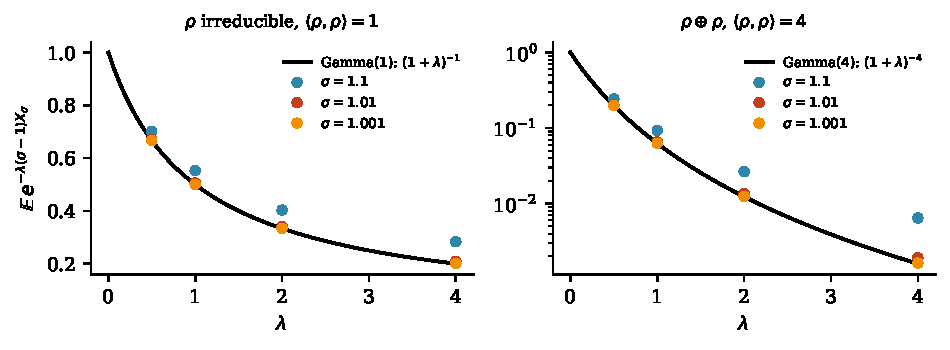
\includegraphics[width=\textwidth]{figs/recip_gamma.pdf}
\caption{Theorem~\ref{thm:recipgamma}: Laplace transforms of $(\sigma-1)X_\sigma$, computed from the complete product $L(s,\rho\otimes\rho)$, for the $S_3$ representation and for $\rho\oplus\rho$, against the Gamma laws with shapes $1$ and $4$.}\label{fig:recipgamma}
\end{figure}

\section{The swap: primes to zeros, computed from Frobenius}\label{sec:recipswap}

The heat trace $\mathcal W_\pi=k_\pi$ of Chapter~\ref{ch:10d}, a sum of $e^{-x\gamma^2}$ over the pairs of zeros $\frac12\pm i\gamma$ (over $\gamma>0$ under GRH), is a function of the zeros, and for automorphic $\pi$ the explicit formula \eqref{eq:10dweil} expresses it through the primes, as Table~\ref{tab:10dheat} does for $\Delta$. The key point for reciprocity is that the prime expression makes sense for any Galois representation, automorphic or not.

\begin{definition}\label{def:recipheat}
Let $\rho$ be self dual, $\Lambda_\rho(n)$ the coefficients of $-L'/L(s,\rho)$ (so $\Lambda_\rho(p^m)=a_\rho(p^m)\log p$ at unramified $p$), and $\gamma(s,\rho)$, $N_\rho$ its gamma factor and conductor. For $x>0$ the \emph{Galois heat trace}\index{heat trace} is
\[
\begin{split}
\mathcal W_\rho(x)={}&\frac1{4\pi}\int_{\R}e^{-xt^2}\Bigl(\log N_\rho+2\operatorname{Re}\frac{\gamma'}{\gamma}\bigl(\tfrac12+it,\rho\bigr)\Bigr)dt\\
&-\frac1{2\pi}\sum_{n\ge2}\frac{\Lambda_\rho(n)}{\sqrt n}\sqrt{\frac\pi x}\,e^{-(\log n)^2/(4x)}.
\end{split}
\]
\end{definition}

The series converges absolutely for every $x>0$, since $|\Lambda_\rho(n)|\le\dim\rho\cdot\log n$ for an Artin representation (more generally $|\Lambda_\rho(n)|\le\dim\rho\cdot n^{\theta}\log n$ when the Satake parameters at every $p$ are bounded by $p^{\theta}$) and the Gaussian factor decays faster than any power of $n$. So $\mathcal W_\rho$ is defined from Frobenius traces, the conductor and the gamma factor alone, with no analytic continuation. To accuracy about $e^{-A}$ only the prime powers with $\log n\le x+\sqrt{x^2+4xA}$, about $\sqrt{4xA}$ for small $x$, matter, so small $x$ needs few primes.

\begin{theorem}[Holomorphy and GRH from the Galois heat trace; this book, after Weil \cite{weil1952,weil1972}]\label{thm:recipcm}
Let $\rho$ be self dual, and suppose $\Lambda(s,\rho)$ has meromorphic continuation of finite order with $\Lambda(s,\rho)=\pm\Lambda(1-s,\rho)$. Write its zeros and poles as $\frac12\pm i\gamma$. Then:
\begin{enumerate}
\item[(i)] $\mathcal W_\rho(x)=\frac12\sum_{\text{zeros}}e^{-x\gamma^2}-\frac12\sum_{\text{poles}}e^{-x\gamma^2}$, with multiplicity, the sums absolutely convergent for $x>0$.
\item[(ii)] $\mathcal W_\rho$ is completely monotone on $(0,\infty)$ if and only if $\Lambda(s,\rho)$ is entire and all its zeros lie on $\operatorname{Re}s=\frac12$.
\end{enumerate}
In particular, for an Artin representation with real character and no trivial constituent (a trivial constituent of multiplicity $r$ adds the pole term $-re^{x/4}$), Artin's conjecture together with GRH for $L(s,\rho)$ is equivalent to the complete monotonicity of a function computed from Frobenius traces.
\end{theorem}

\begin{proof}
(i) is Weil's explicit formula \cite{weil1952} (see \cite{iwanieckowalski2004}, Theorem~5.12) for the even test function $h(t)=e^{-xt^2}$, whose Fourier transform is $\sqrt{\pi/x}\,e^{-u^2/(4x)}$; $h$ is entire and decays in every horizontal strip, so the contour shifts are justified, and poles enter with the opposite sign to zeros. Self duality makes the prime side real and equal to $-\frac1\pi\sum\Lambda_\rho(n)n^{-1/2}\hat h(\log n)$.

(ii) If $\Lambda$ is entire with all $\gamma$ real, (i) exhibits $\mathcal W_\rho$ as the Laplace transform of the positive measure $\frac12\sum\delta_{\gamma^2}$, as in Theorem~\ref{thm:10bmain}(d), which is the automorphic case. Conversely let $\mathcal W_\rho$ be completely monotone, so $\mathcal W_\rho(x)=\int_{[0,\infty)}e^{-xu}\mu(du)$ with $\mu\ge0$ by Bernstein's theorem. Write (i) as $\sum_kc_ke^{-xw_k}$ with distinct $w_k=\gamma_k^2\in\C$ and nonzero weights $c_k$, half the multiplicity, negative for poles. A pole and a zero cannot share a value of $w$: by the functional equation the zero and pole sets are each symmetric under $\gamma\mapsto-\gamma$, and $\gamma^2$ determines $\gamma$ up to sign. All zeros and poles lie in $0\le\operatorname{Re}s\le1$, by the Euler product and the functional equation, so $|\operatorname{Im}\gamma_k|\le\frac12$ and $\operatorname{Re}w_k\ge-\frac14$. Since $\Lambda$ has finite order, the numbers of zeros and poles with $|\gamma|\le T$ grow at most polynomially in $T$, so $\sum_k|c_k|e^{-x\operatorname{Re}w_k}\ll x^{-A}$ as $x\to0$ for some $A$. Fix an integer $M>A+1$. The transform
\[
J(s)=\int_0^\infty e^{-sx}x^M\mathcal W_\rho(x)\,dx
\]
converges for $\operatorname{Re}s$ large, and integrating term by term in each representation,
\[
J(s)=\sum_k\frac{M!\,c_k}{(s+w_k)^{M+1}}=\int_{[0,\infty)}\frac{M!\,\mu(du)}{(s+u)^{M+1}}.
\]
The series converges absolutely and locally uniformly off the points $-w_k$, because $|w_k|\asymp|\gamma_k|^2$ and the counting function grows polynomially, so it defines a meromorphic function on $\C$ with a pole of order $M+1$ at each $-w_k$. The integral is holomorphic on $\C\setminus(-\infty,0]$. Since the two agree for $\operatorname{Re}s$ large, they agree everywhere, so every $-w_k$ lies in $(-\infty,0]$: every $w_k$ is real and nonnegative. With real exponents, uniqueness of the Laplace transform of measures on $[0,\infty)$ gives $\mu=\sum c_k\delta_{w_k}$, so every $c_k$ is positive. Hence there are no poles, so $\Lambda$ is entire, and every $\gamma_k$ is real, since $\gamma_k^2=w_k\ge0$.
\end{proof}

Complete monotonicity is a positivity condition on infinitely many derivatives, but each instance $(-1)^j\mathcal W_\rho^{(j)}(x)\ge0$ is a finite computation with Frobenius traces. A pair of poles of $\Lambda$ at $\frac12\pm iT$ contributes $-e^{-xT^2}$, but it is invisible near $x=T^{-2}$: there the prime sum is of order $Te^{-(T\log2)^2/4}$, so $\mathcal W_\rho(T^{-2})$ is fixed by the conductor and the gamma factor, and as soon as there are ordinates in $(\frac12T,T)$ and in $(T,\frac32T)$ they outweigh the pole term in every inequality $(-1)^j\mathcal W_\rho^{(j)}(T^{-2})\ge0$. A pole midway between consecutive ordinates $2\delta$ apart first violates an inequality near $x=j/T^2$ with $j\approx\frac{\log2}2(T/\delta)^2$ (Exercise~\ref{ex:recippole}). So the inequalities can disprove Artin's conjecture or GRH for $\rho$, one violation at a time, but no finite set of them is known to verify either to any finite height. Booker's verification of Artin's conjecture to finite height \cite{booker2006} combines a group theoretic criterion with the location of zeros by the explicit formula and Turing's method.

The swap is also rigid.

\begin{proposition}[The swap sees every prime; this book]\label{prop:reciprigid}
Let $\rho$ satisfy the conclusion of Theorem~\ref{thm:recipcm}(ii), and let $\rho'$ be self dual Galois data with the same conductor and the same gamma factor, whose local factors differ from those of $\rho$ at a nonempty set $P$ of primes with $\sum_{p\in P}p^{-1/2}\log p<\infty$; suppose that the Satake parameters of $\rho$ and $\rho'$ have absolute value at most $1$. Then $\mathcal W_{\rho'}$ is not completely monotone. In particular, if $\Lambda(s,\rho')$ has meromorphic continuation of finite order with $\Lambda(s,\rho')=\pm\Lambda(1-s,\rho')$, it has a pole or a zero off the critical line.
\end{proposition}

\begin{proof}
By the cosine form \eqref{eq:recipcospair} of the Laplace pair \eqref{eq:10dpair},
\[
\mathcal W_{\rho'}(x)-\mathcal W_\rho(x)=\int_0^\infty e^{-xz}g(z)\,dz,
\]
where $c_{p,m}=\Lambda_{\rho'}(p^m)-\Lambda_\rho(p^m)$ and
\[
g(z)=-\frac1{2\pi\sqrt z}\sum_{p\in P}\sum_{m\ge1}\frac{c_{p,m}}{p^{m/2}}\cos(\sqrt z\,m\log p).
\]
By hypothesis the coefficients are absolutely summable, so $\sqrt z\,g(z)$ is a nonzero uniformly almost periodic function of $r=\sqrt z$ with distinct frequencies $m\log p$ (unique factorisation) and no constant term. If $\mathcal W_{\rho'}$ were completely monotone it would be the Laplace transform of $\mu'\ge0$, and by uniqueness $\mu'=\frac12\sum\delta_{\gamma^2}+g(z)dz$. The absolutely continuous part of a positive measure is nonnegative, so $g\ge0$ almost everywhere. But a nonzero almost periodic function with mean zero takes negative values on a set of positive measure.
\end{proof}

Compare Proposition~\ref{prop:01limits}: altering Frobenius data on a set of primes of density zero changes no distributional statement, but by Proposition~\ref{prop:reciprigid} it destroys the Galois heat trace whenever $\sum_{p\in P}p^{-1/2}\log p<\infty$; a single prime suffices.

Figure~\ref{fig:recipheat} tests this on the $S_3$ representation of conductor $23$, which is automorphic (it is the weight one form $\eta(z)\eta(23z)$; its first zero, $\gamma_1=5.1157$, and its Thorin data are in Table~\ref{tab:10bcatalogue}). The Galois heat trace was computed from Frobenius classes obtained by factoring $x^3-x-1$ modulo primes below $60000$, with no use of the modular form. It agrees with the sum over the zeros of $L(s,\rho)$ to all $16$ digits at $x=0.02$ (both give $1.4102560772724$), to an absolute error of $1.5\cdot10^{-16}$ at $x=0.3$ and to $10^{-8}$ relative at $x=0.7$, where double precision runs out. With the class of $\Frob_2$ changed from order three to the identity, the same function becomes negative from $x=0.1$ on ($-0.32$ at $x=0.1$, $-0.62$ at $x=0.5$), so it is not even positive, let alone completely monotone.

\begin{figure}[t]
\centering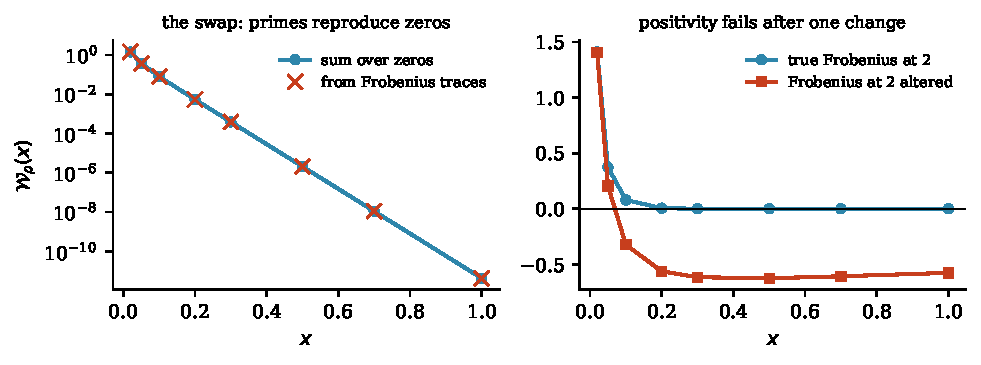
\includegraphics[width=\textwidth]{figs/recip_heat.pdf}
\caption{Left: the Galois heat trace of Definition~\ref{def:recipheat} for the $S_3$ representation, computed from Frobenius classes alone (crosses), against the sum over zeros (line). Right: changing the Frobenius class at $2$ makes it negative.}\label{fig:recipheat}
\end{figure}

\section{Van Dantzig duality and the Euler half line}\label{sec:recipvdp}

For a self dual $\Lambda$ with centre $\frac12$, $\Lambda(\frac12)\ne0$ and a nonnegative P\'olya kernel, the van Dantzig pair of Theorem~\ref{thm:10dvdp}, which exists exactly under GRH, is
\[
f_\Lambda(t)=\frac{\Lambda(\frac12+it)}{\Lambda(\frac12)},\qquad g_\Lambda(t)=\frac{\Lambda(\frac12)}{\Lambda(\frac12+t)} .
\]
The first member lives on the critical line, where by \eqref{eq:recipmellin} it is the Fourier transform of the P\'olya kernel, that is of the automorphic form on $i\R_{>0}$. The second lives on the real axis, and for $t>\frac12$ it is the reciprocal of an Euler product times the central value $\Lambda(\frac12)$, that is Galois data up to one constant. The van Dantzig involution $F\mapsto1/F(i\,\cdot)$ passes between the two faces, and the Wald couple $(W,H)$ of Theorem~\ref{thm:10dvdp}(c), with $\E e^{sW}=\Lambda(\frac12+s)/\Lambda(\frac12)$ and $\E e^{-s^2H}=\Lambda(\frac12)/\Lambda(\frac12+s)$, pairs a variable whose density is the automorphic form with a generalized gamma convolution whose transform is the Euler product. This suggests reading reciprocity as the existence of a Wald couple whose two members are built on different sides; the next theorem makes one direction precise, using only the Euler half line.

\begin{theorem}[Euler half line criterion; this book]\label{thm:recipeuler}
Let $\rho$ be self dual with completion $\Lambda(s,\rho)$, defined for $\operatorname{Re}s>1$ by its Euler product, and let $s_0>\frac14$. Suppose that for $s>\frac14$,
\[
\frac{\Lambda(\frac12+\sqrt{s_0},\rho)}{\Lambda(\frac12+\sqrt s,\rho)}=C\,\E e^{-sH}
\]
for a constant $C>0$ and a generalized gamma convolution $H$ whose Thorin measure is $\sum_kc_k\delta_{u_k}$ with positive integers $c_k$ and $u_k>0$. Then $\Lambda(s,\rho)$ extends to an entire function of finite order, $\Lambda(s,\rho)=\Lambda(1-s,\rho)$, every zero lies on $\operatorname{Re}s=\frac12$, and $\Lambda$ is bounded in vertical strips. Conversely, if $\Lambda(s,\rho)$ is entire of order one with this functional equation, $\Lambda(\frac12,\rho)\ne0$ and all zeros on the critical line, then the hypothesis holds with $u_k=\gamma_k^2$.
\end{theorem}

\begin{proof}
A GGC with drift $a\ge0$ and Thorin measure $\sum c_k\delta_{u_k}$ has $\E e^{-sH}=e^{-as}\prod_k(1+s/u_k)^{-c_k}$, with $\sum_kc_k/u_k<\infty$. Since the $c_k$ are positive integers, $E(z)=e^{az^2}\prod_k(1+z^2/u_k)^{c_k}$ is an even entire function of $z$ of finite order. For real $z>\frac12$ we have $\Lambda(\frac12+z,\rho)=C^{-1}\Lambda(\frac12+\sqrt{s_0},\rho)E(z)$, and both sides are holomorphic on $\operatorname{Re}z>\frac12$, so they agree there; the right side provides the continuation of $\Lambda(\frac12+z,\rho)$ to an entire function. Evenness of $E$ is the functional equation, and the zeros of $E$ are at $z=\pm i\sqrt{u_k}$, that is $s=\frac12\pm i\sqrt{u_k}$. On $\operatorname{Re}s=1+\delta$ the completion is bounded because the gamma factor decays and the Euler product is bounded; by the functional equation the same holds on $\operatorname{Re}s=-\delta$; finite order and the Phragm\'en Lindel\"of principle give boundedness in the strip between. The converse is Theorem~\ref{thm:10dduality} applied to $\Lambda(\frac12+z,\rho)$, normalised at $z=\sqrt{s_0}$ instead of $0$.
\end{proof}

Combining Theorem~\ref{thm:recipeuler} with Proposition~\ref{prop:recipsym}, we obtain a Thorin form of Hecke's converse theorem.

\begin{corollary}[Thorin converse theorem at level one; this book]\label{cor:recipconverse}
Let $k\equiv0\bmod4$ and let $(a_p)$ be the Frobenius traces of a self dual Galois representation of conductor $1$ with the gamma factor $\Gamma_{\C}(s+\frac{k-1}2)$, where $\Gamma_\C(s)=\Gamma_\R(s)\Gamma_\R(s+1)=2(2\pi)^{-s}\Gamma(s)$, and Ramanujan bound, with $a_n$ its Dirichlet coefficients. If the normalised Euler product $\Lambda(\frac12+\sqrt{s_0})/\Lambda(\frac12+\sqrt s)$, $s>\frac14$, is a constant times the Laplace transform of a GGC whose Thorin measure is a sum of point masses with positive integer weights, then $\sum a_nn^{(k-1)/2}e^{2\pi inz}$ is a cusp form of weight $k$ for $\SL_2(\Z)$, and it satisfies GRH.
\end{corollary}

\begin{proof}
By Theorem~\ref{thm:recipeuler} the completion is entire, bounded in vertical strips and even about the centre. In the classical normalisation (centre $\frac k2$) this is $\Lambda(k-s)=\Lambda(s)=(-1)^{k/2}\Lambda(s)$, which is (iii) of Proposition~\ref{prop:recipsym} with $N=1$, so $f$ is a cusp form.
\end{proof}

The hypothesis of Corollary~\ref{cor:recipconverse} is stated entirely on the Euler half line, so it is a statement about Galois data; it is stronger than reciprocity, since it includes GRH. Its natural weakening, with nonzero integer weights and complex atoms, always holds for the Artin representations of Open Problem~\ref{op:recipsigned}, where Artin's conjecture is the positivity of the weights.

\subsection{An unconditional Galois family}

Positivity is available unconditionally on the Galois side whenever the logarithmic coefficients are nonnegative, as for Dedekind zeta functions; the case used here is the Rankin Selberg square. For $\alpha>1$ let $F(s)=\Lambda^S(s,\rho\otimes\check\rho)$, the completion of $D^S$ of Section~\ref{sec:recipgalois}.

\begin{proposition}[this book]\label{prop:recipfamily}
For every Artin representation $\rho$ and every $\alpha>1$ there is a GGC $H_\alpha$ with
\[
\frac{F(\alpha)}{F(\alpha+\sqrt s)}=e^{-b_\alpha\sqrt s}\,\E e^{-sH_\alpha},\qquad b_\alpha=\frac{F'(\alpha)}{F(\alpha)},
\]
whose Thorin density is the $2\sin^2$ transport (Lemma~\ref{lem:10dsin2}) of the measure
\[
\sum_{p\notin S,\,m\ge1}|a_\rho(p^m)|^2(\log p)\,p^{-m\alpha}\delta_{m\log p}
\]
($x$ times the L\'evy measure of $X_\alpha$) together with the gamma factor contribution. It is computed from Frobenius traces alone.
\end{proposition}

\begin{proof}
The function $F$ is holomorphic and zero free on $\operatorname{Re}s>1$. The second derivative of $\log F$ along the real axis is the sum of the trigamma terms of the gamma factor and of $\sum|a_\rho(p^m)|^2(m\log p)^2m^{-1}p^{-ms}$, both completely monotone and tending to zero. Lemma~\ref{lem:10dsin2} applies.
\end{proof}

As $\alpha$ decreases to $1$ the pole of order $\langle\rho,\rho\rangle$ appears (Theorem~\ref{thm:recipgamma}). Below $1$ the Euler product no longer defines $F$. Meromorphic continuation of $L(s,\rho\otimes\check\rho)$ is known for every Artin $\rho$ by Brauer's theorem, and holomorphy away from $s=1$ follows from automorphy of $\rho$ by the Rankin Selberg theory; neither gives positivity. For automorphic $\rho$, apply the argument of Theorem~\ref{thm:10dshift} to the complete function $\Lambda(s,\rho\otimes\check\rho)$, all Euler factors included and the poles at $s=0,1$ removed: its transforms at the base points $\alpha\in(\frac12,1]$ are GGCs, with nonnegative Thorin densities $V_{\alpha-1/2}$, for every such $\alpha$ exactly when GRH holds for $L(s,\rho\otimes\check\rho)$, and the densities then converge to the Thorin measure of the zeros as $\alpha\downarrow\frac12$. For irreducible two dimensional $\rho$ this GRH contains the Riemann hypothesis, since $L(s,\rho\otimes\check\rho)=\zeta(s)L(s,\operatorname{Ad}\rho)$ with $L(s,\operatorname{Ad}\rho)$ entire \cite{gelbartjacquet1978}. Splitting off the factor $e^{-b_\alpha\sqrt s}$ as in Proposition~\ref{prop:recipfamily}, with $b_\alpha$ now the logarithmic derivative of this complete function at $\alpha$, leaves the densities $V_{\alpha-1/2}-b_\alpha/(2\pi\sqrt z)$ (Lemma~\ref{lem:10dsin2}), and their positivity below $\alpha=1$ is not known to follow from GRH; for $\xi$ it follows from the Riemann hypothesis by a theorem of Lagarias, and is not known unconditionally (Section~\ref{sec:10daway}). \emph{Continuing a family of positive measures, defined from Frobenius traces above the line $\operatorname{Re}s=1$, down to the centre while preserving positivity} is the probabilistic form of the problem that this chapter proposes; for the Rankin Selberg square it is holomorphy away from $s=1$ together with GRH for $L(s,\rho\otimes\check\rho)$, which does not by itself give reciprocity.

\section{The programme}\label{sec:recipprogramme}

The equivalences of this chapter prove nothing new about reciprocity; like the Thorin forms of the Riemann hypothesis, they move the difficulty rather than remove it. They offer positivity and symmetry statements about Galois data, to which probabilistic tools apply and which can be tested one prime at a time.
\begin{enumerate}
\item Symmetry. At level one, reciprocity is the evenness (oddness when $k\equiv2\bmod4$) of the P\'olya kernel built from Frobenius traces (Proposition~\ref{prop:recipsym}). At level $N$ it is the pairing of twisted kernels required by Weil's converse theorem.
\item Positivity. For self dual $\rho$ with meromorphic continuation of finite order and a functional equation, holomorphy together with GRH is the complete monotonicity of the Galois heat trace (Theorem~\ref{thm:recipcm}), a function of Frobenius traces each of whose derivatives is computable at each $x$ to any accuracy in finitely many steps. One certified violation disproves holomorphy or GRH; no finite set of verified inequalities is known to prove them to any finite height.
\item Rigidity. The Galois heat trace detects a change of Frobenius data at a single prime (Proposition~\ref{prop:reciprigid}), in contrast with every distributional statement (Proposition~\ref{prop:01limits}).
\item Continuation. On the Euler half line the Galois side produces GGCs, from the Rankin Selberg square unconditionally (Proposition~\ref{prop:recipfamily}) and from $\rho$ itself under the Thorin hypothesis (Theorem~\ref{thm:recipeuler}). Holomorphy together with GRH, for $L(s,\rho\otimes\check\rho)$ in the first case and for $L(s,\rho)$ in the second, is the continuation to the centre of the corresponding GGCs (for the Rankin Selberg square with its poles removed and the drift kept inside, as in Theorem~\ref{thm:10dshift}); at level one the second gives reciprocity (Corollary~\ref{cor:recipconverse}).
\item Laws. On the Frobenius probability space reciprocity is almost sure equality, and its uniqueness statements, the correspondence of irreducible with cuspidal and, for every $\epsilon>0$, agreement within $\epsilon$ outside a set of primes of Dirichlet density zero follow from two orthonormality theorems (Corollary~\ref{cor:reciplaw}); class field theory is measurability with respect to congruences (Proposition~\ref{prop:recipcongruence}). Laws cannot give existence; the objects of items 1 to 3 see individual primes, but they too give existence only through a converse theorem.
\item Gamma processes. Equidistribution of Frobenius data is a Gamma process limit of the labelled factorisation of a random integer (Theorem~\ref{thm:recipgammaproc}); reciprocity laws are vanishing statements for Thorin measures (Theorem~\ref{thm:recipthorin}); and comparing an Artin representation with a cuspidal one gives a conjectured zero two law (Conjecture~\ref{conj:recipmixed}), the orthogonality half of reciprocity: it is implied by reciprocity and asserts no existence, and the existence of a partner is the other half.
\item Gaussian model. For $\GL_1$ the symmetry part of the programme runs, and the circle models the positivity part: the theta transformation, proved from the normal characteristic function or by Fej\'er positivity of the winding number terms, gives quadratic reciprocity and Gauss's sign (Section~\ref{sec:recipgauss}).
\item Irreducibility. The Gamma shape of the Rankin Selberg subordinator is $\langle\rho,\rho\rangle$ (Theorem~\ref{thm:recipgamma}), the probabilistic shadow of ``irreducible corresponds to cuspidal''.
\end{enumerate}

The most concrete target is the even icosahedral case, where reciprocity is open and the Galois data are explicit. For such $\rho$ every quantity above can be computed from the Frobenius classes. Factorisation patterns modulo $p$ give these only up to Galois conjugacy, so they cannot tell apart the two classes of elements of order $5$ in the projective image $A_5$, on whose preimages the traces of $\rho$ differ; a Frobenius resolvent separates them \cite{dokchitser2013}. When $\det\rho$ is trivial, so that $\rho$ is self dual, item~2 tests Artin's conjecture together with GRH (Problem~\ref{cp:recipicosa}). The analogue of Proposition~\ref{prop:recipsym} for the gamma factor $\Gamma_\R(s)^2$ or $\Gamma_\R(s+1)^2$ of an even representation (as complex conjugation acts by $1$ or $-1$), with a $K$ Bessel kernel in place of the exponential, gives symmetry tests for the twisted kernels.

\subsection{Open problems}

\begin{problem}[The Thorin converse theorem in general]\label{op:recipgln}
Formulate and prove a version of Theorem~\ref{thm:recipeuler} for twists $\rho\times\pi'$ that are not self dual, strong enough to combine with the converse theorem of Cogdell and Piatetski Shapiro. The obstacle is that the completion $\Xi_\rho$ of Definition~\ref{def:10bxi}, built from $\Lambda(\frac12+z,\rho)\Lambda(\frac12+z,\check\rho)$, controls the product of two $L$ functions, whereas converse theorems need each one.
\end{problem}

\begin{problem}[Descending the base point]\label{op:recipdescent}
For automorphic $\rho$, positivity of the densities $V_{\alpha-1/2}$, with the drift kept inside, for every $\alpha\in(\frac12,1]$ is GRH for $L(s,\rho\otimes\check\rho)$ (end of Section~\ref{sec:recipvdp}). Decide whether the densities $V_{\alpha-1/2}-b_\alpha/(2\pi\sqrt z)$ of that section, with the drift split off, also stay nonnegative there, which for $\xi$ holds under the Riemann hypothesis and is proved unconditionally for $\alpha\ge1$ (Section~\ref{sec:10daway}) and for $\frac12<\alpha<1$ below height $3\times10^{12}$ (Chapter~\ref{ch:beta}), and identify the obstruction to positivity below $\alpha=1$ in terms of Frobenius data alone: which features of the L\'evy measure of $X_\alpha$ at $\alpha>1$ control the sign of the transported density at $\alpha<1$? For $\xi$ and $\Delta$ the computational counterpart is the problem on transported Thorin densities in the strip in Chapter~\ref{ch:10d}.
\end{problem}

\begin{problem}[Signed Thorin measures]\label{op:recipsigned}
For an Artin representation $\rho$ with real character, no trivial constituent, root number $1$ and $\Lambda(\frac12,\rho)$ finite and nonzero, Brauer's theorem and Hadamard factorisation give, for a fixed $s_0>\frac14$, $\Lambda(\frac12+\sqrt{s_0},\rho)/\Lambda(\frac12+\sqrt s,\rho)=C\prod_k(1+s/u_k)^{-c_k}$ with nonzero integers $c_k$ and complex $u_k=\gamma_k^2$, where $c_k<0$ exactly at poles, and $u_k\notin(0,\infty)$ exactly at zeros and poles off the critical line. Artin's conjecture for $\rho$ is the statement that every $c_k$ is positive. Find a property of the signed L\'evy measure of $\log\Lambda(s,\rho)$ on the Euler half line, that is of Frobenius data, which forces every $c_k$ to be positive without forcing the $u_k$ to be real, so that holomorphy is separated from GRH (compare Section~\ref{sec:10bparabola}).
\end{problem}

\begin{problem}[A Fej\'er summation for primes]\label{op:recipfejer}
Find positive weights $w_N(n)\le1$ with $w_N(n)\to1$ such that the prime side of Definition~\ref{def:recipheat}, with $\Lambda_\rho(n)$ replaced by $w_N(n)\Lambda_\rho(n)$ and the archimedean term adjusted accordingly, is the Laplace transform of a positive measure, and such that positivity for each $N$ follows from Frobenius data alone, as Fej\'er positivity does for the circle (Proposition~\ref{prop:recipfejer}); otherwise $w_N\equiv1$ works whenever holomorphy and GRH hold. By Theorem~\ref{thm:recipcm} this would prove holomorphy and GRH for $L(s,\rho)$; the problem is to see what positivity of this kind forces on Frobenius data (compare Open Problem~\ref{op:thorin}).
\end{problem}

\begin{problem}[Reciprocity in law versus reciprocity]\label{op:reciplaw}
Show that if an irreducible Artin representation $\rho$ is reciprocal in law with a cuspidal $\pi$ (Corollary~\ref{cor:reciplaw}), then $a_\rho(p)=a_\pi(p)$ for all but finitely many $p$ (compare Open Problem~\ref{op:inverse} and Corollary~\ref{cor:01functional}). It holds whenever $\rho$ is known to be automorphic, by Corollary~\ref{cor:reciplaw}(v); for $n=2$, where this leaves the even icosahedral $\rho$, it would follow from a refinement of Ramakrishnan's theorem \cite{ramakrishnan1994} to the case in which one member is Galois and the agreement is only approximate, as in Corollary~\ref{cor:reciplaw}(iv); in general it is a strong multiplicity one statement across the two sides.
\end{problem}

\begin{problem}[The mixed zero two law]\label{op:recipmixed}
Show that meromorphy of $L(s,\rho\times\tilde\pi)$ near $\operatorname{Re}s=1$, with at most a simple pole at $s=1$ and no zeros on the line, gives the dichotomy of Conjecture~\ref{conj:recipmixed} by the argument of Theorem~\ref{thm:recipzerotwo} and reduces the rest of the conjecture to a form of Open Problem~\ref{op:reciplaw}, and prove the conjecture for one even icosahedral Artin representation.
\end{problem}

\begin{problem}[Joint marked processes]\label{op:recipjoint}
Show that the joint limit of the marked processes of Theorem~\ref{thm:recipgammaproc} exists for an Artin representation $\rho$ and a cuspidal $\pi$ of the same dimension; it is not determined by the two marginal limits (compare Exercise~\ref{ex:recipjoint} and Theorem~\ref{thm:04joint}). Is the joint label law either supported on $\{a_\rho=a_\pi\}$, or such that the Thorin measure of $|a_\rho-a_\pi|^2$ has mass bounded below by a constant depending only on $n$?
\end{problem}

\begin{problem}[Signs of drifts]\label{op:recipdrift}
When does the split class approach its Gamma limit from above, $\kappa_{\{1\}}<0$ in Theorem~\ref{thm:recipdrift}? This requires $\gamma_K^S<0$. Characterise such fields and relate the signs of the $\kappa_C$ to the bias between classes that Section~\ref{sec:ch3cheb} measures for the field of Example~\ref{ex:ch3cubic} (Exercise~\ref{ex:ch3fs}), and to the Chebotarev races of the computational problems of Chapter~\ref{ch:03}.
\end{problem}

\section{Notes}

Reciprocity in the form used here is from Langlands' letter and lectures \cite{langlands1967,langlands1970}; the known cases cited are \cite{langlands1980,tunnell1981,wiles1995,taylorwiles1995,bcdt2001,kharewintenberger2009,kharewintenberger2009b,kisin2009}; potential automorphy is from \cite{hsbt2010,blght2011} and symmetric power functoriality from \cite{newtonthorne2021,newtonthorne2021b}. Artin's conjecture and Brauer's theorem are \cite{artin1924,brauer1947}, and Artin's reciprocity law is \cite{artin1927}. Converse theorems are due to Hecke \cite{hecke1936}, Weil \cite{weil1967}, Jacquet and Langlands \cite{jacquetlanglands1970} and Cogdell and Piatetski Shapiro \cite{cogdellps1994}. The Rankin Selberg pole is from Jacquet and Shalika \cite{jacquetshalika1981} and Moeglin and Waldspurger \cite{moeglinwaldspurger1989}. Theorem~\ref{thm:recipcm}(ii) is Weil's positivity criterion \cite{weil1952,weil1972} restricted to the test functions $t^{2j}e^{-xt^2}$; Weil's extension of the explicit formula to Artin Hecke $L$ functions \cite{weil1972} already ties positivity to Artin's conjecture together with GRH. The Thorin framework for automorphic $L$ functions of Chapters~\ref{ch:10b} to \ref{ch:10d} extends the first author's work \cite{polson2017,polson2018vdp}; the sine squared lemma is Lemma~14 of \cite{polson2018vdp}, with its first step from Roynette and Yor \cite{roynetteyor2005}, who also introduced Wald couples with infinitely divisible members; van Dantzig pairs and Wald couples for $\xi$ are in \cite{roynetteyor2005,polson2018vdp,konstantopoulospatiesarkar2024}. The theta transformation goes back to Jacobi and Poisson; reciprocity for Gauss sums is due to Schaar \cite{schaar1850} and Landsberg \cite{landsberg1893}, and the derivation of quadratic reciprocity from it is in Dym and McKean \cite{dymmckean1972}. Our proofs in Section~\ref{sec:recipgauss} differ only in reading Poisson summation as the Fourier series of a wrapped normal law and Fej\'er's proof of it as a Laplace transform through the pair of the $2\sin^2$ lemma (Proposition~\ref{prop:recipfejer}). Zolotarev's proof \cite{zolotarev1872}, through signs of permutations, is another short route to Corollary~\ref{cor:recipqr}. Dedekind sums and their reciprocity law are treated in \cite{rademachergrosswald1972}. Poisson random measures and the Gamma process are in Kingman \cite{kingman1993}, the Dirichlet process in Ferguson \cite{ferguson1973}, and generalized gamma convolutions in Thorin \cite{thorin1977} and Bondesson \cite{bondesson1992}. Sato Tate for newforms and its joint form are \cite{blght2011,harris2009}. Euler Kronecker constants are Ihara's \cite{ihara2006}; negative values for cyclotomic fields are in \cite{fordlucamoree2014}. Ours are Theorems~\ref{thm:recipgammaproc}, \ref{thm:recipggcfun}, \ref{thm:recipthorin}, \ref{thm:recipzerotwo} and \ref{thm:recipdrift} in the forms stated, the bounds (i) and (ii) of Theorem~\ref{thm:recipheat}, Corollary~\ref{cor:recipchebgamma}, Conjecture~\ref{conj:recipmixed} with Proposition~\ref{prop:recipmixed}, the probabilistic formulations of Section~\ref{sec:reciplaw}, Corollary~\ref{cor:reciplaw}, Proposition~\ref{prop:recipcongruence} (a reformulation of Chebotarev's theorem for $K(\zeta_N)$), Proposition~\ref{prop:recipsym} in this form, Theorem~\ref{thm:recipgamma}, Definition~\ref{def:recipheat}, Theorem~\ref{thm:recipcm}, Proposition~\ref{prop:reciprigid}, Theorem~\ref{thm:recipeuler}, Corollary~\ref{cor:recipconverse}, Proposition~\ref{prop:recipfamily} and the computations; each rests on the cited theory.

\section{Exercises}

\begin{enumerate}
\item\label{ex:recipdelta} Show that the kernel $\Phi_f$ of \eqref{eq:recipmellin} for $f=\Delta$ is $\Lambda(6,\Delta)\Phi_\Delta$, with $\Phi_\Delta$ the normalised kernel of Chapters~\ref{ch:02} and \ref{ch:10}, so that its evenness, proved there, is the case $N=1$, $k=12$ of Proposition~\ref{prop:recipsym}. For a newform $f$ of level $N$ and trivial character, and a primitive character $\chi$ modulo $q$ with $(q,N)=1$, write the relation between $\Phi_{f\otimes\chi}(-u)$ and $\Phi_{f\otimes\bar\chi}(u)$ that Weil's converse theorem requires, with its constant.
\item\label{ex:recipshape} For the $S_3$ representation $\rho$ of $x^3-x-1$, show that $\rho\otimes\rho\cong\mathsf{1}\oplus\operatorname{sgn}\oplus\rho$ and $L(s,\rho\otimes\rho)=\zeta(s)L(s,\chi_{-23})L(s,\rho)$, and deduce the shape $1$ in Theorem~\ref{thm:recipgamma}. What is the shape for $\mathsf{1}\oplus\operatorname{sgn}$?
\item\label{ex:recipgauss} Identify, prime by prime, the Laplace transform in Proposition~\ref{prop:reciprigid} with the oscillatory part of a local Thorin comb (Proposition~\ref{prop:10cdictionary}). Compare it with the winding number terms of Proposition~\ref{prop:recipfejer}: why do the cosine densities of all winding numbers, summed with Fej\'er weights, give point masses, while those of the powers of a single prime give a signed density?
\item\label{ex:recippole} Suppose $\Lambda(s,\rho)$ has simple poles at $\frac12\pm iT$, $\Lambda(\frac12,\rho)\ne0$, and is otherwise as in GRH, with positive ordinates $\gamma_1<\gamma_2<\cdots$. Show that $\mathcal W_\rho(x)<0$ for all large $x$ if $T<\gamma_1$. If $\frac12T<\gamma_n<T<\gamma_{n+1}<\frac32T$, show that every inequality $(-1)^j\mathcal W_\rho^{(j)}(T^{-2})\ge0$ holds, but that $(-1)^j\mathcal W_\rho^{(j)}(j/T^2)<0$ for all large $j$; when $T$ is the midpoint and $2\delta=\gamma_{n+1}-\gamma_n$ is small compared with $T$, the least such $j$ is about $\frac{\log2}2(T/\delta)^2$. (For the $S_3$ representation of conductor $23$ and $T$ midway between $\gamma_1$ and $\gamma_2$ the first violation is at $j=13$, near $x=13.5/T^2$.)
\item\label{ex:recipgenls} Apply Lemma~\ref{lem:recipwrap} with $y\ne0$ in the proof of Theorem~\ref{thm:recipls} to obtain reciprocity for $\sum_{n\bmod c}e^{\pi i(an^2+bn)/c}$ when $ac+b$ is even.
\item\label{ex:recipdedekind} Let $K$ be uniform on $\Z/c\Z$, let $((x))=x-\lfloor x\rfloor-\frac12$ for $x\notin\Z$ and $((x))=0$ otherwise, and let $s(b,c)=\sum_{k\bmod c}((k/c))((bk/c))$ be the Dedekind sum. Show that $s(b,c)$ is $c$ times the covariance of $((K/c))$ and $((bK/c))$, and that for $U$ uniform on $[0,1)$ the covariance of $((bU))$ and $((cU))$ is $1/(12bc)$ when $\gcd(b,c)=1$. Explain why this does not yet give Dedekind's reciprocity law $s(b,c)+s(c,b)=\frac{b^2+c^2+1}{12bc}-\frac14$. A probabilistic proof of the reciprocity law, and an extension of Theorem~\ref{thm:recipheat} to the Dedekind eta function, whose multiplier involves Dedekind sums, are left open.
\item\label{ex:recipjoint} For the $S_3$ representations $\rho$ and $\rho_{31}$ of the text, compute the limiting joint law of $(a_\rho,a_{\rho_{31}})$ and check that $d(\rho,\rho_{31})^2=2$. What is the joint law for $\rho$ and $\rho\otimes\chi_{-23}$, and what is $d$?
\item\label{ex:recipwald} Show that for $s>\frac12$ the Wald couple identity $\E e^{sW}\E e^{-s^2H}=1$ involves $\Lambda$ only through the Euler product values $\Lambda(\frac12+s)$ and the single central value $\Lambda(\frac12)$. Show that a random variable $W$ with $\E e^{sW}=\Lambda(\frac12+s)/\Lambda(\frac12)$ for all $s>\frac12$, if it exists, has its law determined by these values (tilt by $e^{s_0W}$ with $s_0>\frac12$), and explain why the identity on $s>\frac12$ cannot by itself show that such a $W$ exists.
\end{enumerate}

\section{Open computational problems}

\begin{compproblem}[Even icosahedral representations]\label{cp:recipicosa}
Objective: for an icosahedral Artin representation $\rho$ with trivial determinant (hence self dual and even) from the LMFDB, compute the Galois heat trace of Definition~\ref{def:recipheat} and its derivatives in ball arithmetic and search for a certified violation of $(-1)^j\mathcal W_\rho^{(j)}(x)\ge0$, which by Theorem~\ref{thm:recipcm} would disprove Artin's conjecture or GRH for $\rho$. Objects and scale: one representation, prime powers up to $10^{10}$, orders $j\le10^3$ and $x\in[0.01,4]$, where these primes suffice to certify signs (beyond $x\approx5$ the omitted prime powers can outweigh the inequalities); a pole at height $T$ midway between ordinates $2\delta$ apart would first show near $x=j/T^2$ with $j\approx\frac{\log2}2(T/\delta)^2$, that is near $x=\frac{\log2}{2\delta^2}$, so this range reaches it only for $\delta$ above about $0.3$ and $T\le54\delta$, which at conductors of a few million, as in the LMFDB examples, leaves the lowest gaps and unusually wide ones. Route: Frobenius classes from the factorisation of the defining polynomial modulo primes, with a Frobenius resolvent \cite{dokchitser2013} separating the two Galois conjugate classes of order $5$ and the two of order $10$, and archimedean integrals in Arb; the same computation for newforms is the problem on monotonicity across weights and levels in Chapter~\ref{ch:10}. Deliverable: certified signs on the grid, and the region of $(T,\delta)$ in which a pole would have been detected, compared with Booker's finite height verifications \cite{booker2006}. Why it matters: it evaluates the swap on a representation whose automorphy is unknown; satisfied inequalities are not known to verify Artin's conjecture or GRH.
\end{compproblem}

\begin{compproblem}[Kernel symmetry at level $N$]\label{cp:recipkernel}
Objective: test the twisted kernel symmetries required by Weil's converse theorem for Galois data of conductor up to $10^4$ (Artin representations and elliptic curves from the LMFDB), and measure how quickly a change of Frobenius at one prime is detected as a function of that prime. This extends the computational problems on functional equations as a test statistic (Chapter~\ref{ch:02}) and on detecting impostors (Chapter~\ref{ch:01}) to twisted kernels and Artin representations. Route: twisted kernels $\Phi_{f\otimes\chi}$ from $q$ expansions (for even Artin representations, with the $K$ Bessel kernel of their gamma factor), with coefficients from the LMFDB or from Frobenius data, for primitive $\chi$ of conductor up to $50$ prime to $N$, checked against PARI/GP \texttt{lfun}. For even representations the kernels can also be computed from the $L$ function alone, by Bromwich inversion of $\Lambda(s,\rho\otimes\chi)$ on the critical line as in Proposition~\ref{prop:lappolya}, with the gamma factor $\Gamma_\R(s)^2$ or $\Gamma_\R(s+1)^2$; this assumes Artin's conjecture for $\rho\otimes\chi$, and reciprocity predicts that the result is built from a Maass form $u$ of eigenvalue $\frac14$ on the imaginary axis: from $u$ itself for $\Gamma_\R(s)^2$, and from $\partial u/\partial x$, $u$ being odd, for $\Gamma_\R(s+1)^2$. Deliverable: asymmetry tables and detection thresholds. Why it matters: it measures how much of Weil's converse theorem a finite computation sees.
\end{compproblem}

\begin{compproblem}[Gamma process tests at scale]\label{cp:recipgammaproc}
Objective: compute the Thorin measures of Theorem~\ref{thm:recipthorin} and the drifts of Theorem~\ref{thm:recipdrift} for every Galois field of degree at most $10$ in the LMFDB with absolute discriminant below $10^6$, and for pairs of elliptic curves of conductor up to $10^4$. Route: the scripts \texttt{laws.py} and \texttt{second.py} of Table~\ref{tab:B:scripts}, with Frobenius elements from \texttt{idealfrobenius} after \texttt{galoisinit} (which handles every group of order at most $10$) and $a_p$ from \texttt{ellap} in PARI/GP, for primes up to $10^8$. Deliverable: tables of drifts against $\gamma_K$, and of zero probability exponents against Thorin masses. Why it matters: it tests the drift of the split class against Ihara's Euler Kronecker constant and its GRH bound (Theorem~\ref{thm:recipdrift}) on many fields at once.
\end{compproblem}

\begin{compproblem}[Gamma shapes for $\ell$ adic representations]\label{cp:recipgamma}
Objective: estimate the Gamma shape of Theorem~\ref{thm:recipgamma} from Frobenius traces alone, for symmetric powers of elliptic curves and for $\GL_3$ motives, and use it as a statistical test of irreducibility. It is the Dirichlet density counterpart of the Weyl average problems of Chapter~\ref{ch:04}. Route: $a(p)$ from \texttt{ellap} and the symmetric power recursions in PARI/GP for $p\le X=10^9$. Deliverable: shape estimates with confidence intervals at $\sigma-1\ge5/\log X$, after correcting the truncation bias $mE_1((\sigma-1)\log X)$, compared with the direct estimate $\pi(X)^{-1}\sum_{p\le X}|a(p)|^2$ of $m$. Why it matters: the Gamma shape is the probabilistic form of the Rankin Selberg pole order, and the comparison shows how much of it is visible at finite $X$.
\end{compproblem}
